\documentclass[12pt]{article} % Here we state, that we need the text size to be 12p and we want article setup

\usepackage[utf8]{inputenc} % Allows the user to input accented characters directly from the keyboard
\usepackage[T1]{fontenc} % Oriented to output, that is, what fonts to use for printing characters
\usepackage[english]{babel} % The language, you are writing in - you should be able to change to danish

\usepackage[margin=2.5cm]{geometry} % How big margins we want
\geometry{a4paper} % What type of paper we want

\setlength\parindent{0pt} % Makes \noindent standard (my preference - not everyones!)

\usepackage{todonotes} % With this, you can add todo-notes: \todo{stuff todo} or \todo[inline]{stuff todo}
\usepackage{caption} % You can create captions for your tables, pictures etc. AND YOU WANT TO DO THAT
\usepackage{wrapfig} % Allows in-line images if needed
\usepackage{hyperref} % Allows you to create hyperlinks within the document
\hypersetup{colorlinks=false,hidelinks, citecolor=black, urlcolor=black}
\usepackage{url} % Enables typesetting of hyperlinks

\usepackage{amsmath} % Math in your tex 
\usepackage{amsfonts} % Math in your tex 
\usepackage{mathtools} % Math in your tex 
\DeclarePairedDelimiter{\ceil}{\lceil}{\rceil} % Math in your tex 

\usepackage{csquotes} % Provides advanced facilities for inline and display quotations
\usepackage[titletoc]{appendix} % Names appendices "Appendix A" instead of just A in Contents

\usepackage{pdfpages} % We can now import pdf files to our tex file - win!
\usepackage{graphicx} % We can now import pictures - uhlalalah!

\usepackage{algorithm} % http://ctan.org/pkg/algorithms
\usepackage{algpseudocode} % http://ctan.org/pkg/algorithmicx
\usepackage{listings}
\usepackage{color}
\usepackage{graphicx}
\usepackage{lipsum}
\usepackage{cleveref}
\lstset{
    escapeinside={(*@}{@*)},          % if you want to add LaTeX within your code
}

\definecolor{bluekeywords}{rgb}{0.13,0.13,1}
\definecolor{greencomments}{rgb}{0,0.5,0}
\definecolor{turqusnumbers}{rgb}{0.17,0.57,0.69}
\definecolor{redstrings}{rgb}{0.5,0,0}

\lstdefinelanguage{FSharp}
                {morekeywords={let, new, match, with, rec, open, module, namespace, type, of, member, and, for, in, do, begin, end, fun, function, try, mutable, if, then, else},
    keywordstyle=\color{bluekeywords},
    sensitive=false,
    morecomment=[l][\color{greencomments}]{///},
    morecomment=[l][\color{greencomments}]{//},
    morecomment=[s][\color{greencomments}]{{(*}{*)}},
    morestring=[b]",
    stringstyle=\color{redstrings}
    }
\graphicspath{ {images/} } 
\usepackage{natbib} % Bibliography stuff


%-----------------------------------------------------------------------------
% HEADER AND FOOTER STUFF
%-----------------------------------------------------------------------------
\usepackage{fancyhdr}
\usepackage{lastpage} % Making it possible to write ``Page x of y'' in the footer

\pagestyle{fancy}
\fancyhf{}
% Header stuff below
\lhead{Mark Roland Larsen} 
\chead{}
\rhead{fvg932} 
% Footer stuff below
\cfoot{Page \thepage \hspace{1pt} of \pageref{LastPage}} % To the left at the bottom

%-----------------------------------------------------------------------------
\begin{document} % You always need this


\includepdf[pages={-}]{forside.pdf} % How we get our fancy frontpage imported to our file


%-----------------------------------------------------------------------------
% ABSTRACT STUFF (only needed if you have to write this sort of things ;o) )
%-----------------------------------------------------------------------------

%\begin{abstract}
%\noindent 
%\end{abstract}

%-----------------------------------------------------------------------------
% CONTENT STUFF
%-----------------------------------------------------------------------------

\newpage % I want my table of contents on its own page
\tableofcontents
\newpage

%\renewcommand{\abstractname}{Acknowledgements} % If you want to thank someone, this is the way 
%\begin{abstract}
%\noindent 
%\end{abstract}



%-----------------------------------------------------------------------------
% ACTUAL CONTENT STUFF
%-----------------------------------------------------------------------------

\section{Abstract}

\section{Limitations}

I følgende opgave arbejdes der på binære træer med typen 

\section{Introduction}

The string matching problem is found in various fields of study \cite{mit}. In biology, string matching algorithms significantly aid biologists in retrieving and comparing DNA strings, reconstructing DNA strings from overlapping string fragments and looking for new or presented patterns occurring in a DNA\cite{gusfield}. Text-editing applications also adopt string matching algorithms, whenever the application has to acquire an unambiguous occurrences of a user-given pattern, such as a word in some document\cite{introduction, gusfield}. String matching is used in music equipment, AI (artificial intelligence) and in addition, various software applications like virus scanners (anti-virus) or intrusion detection systems, frequently adopt string matching algorithms as a practical tool, to secure data security over the internet \cite{detection}.
Fundamentally, string matching is a method to find some pattern $P =\{p_1,p_2,…,p_n\}$ in a given text $T=\{t_1, t_2,…,t_m\}$, over some finite alphabet $\Sigma$ as illustrated in \cref{fig:banana} \cite{detection}.

\section {String Matching}

Exact string matching is both an algorithmic problem and data structure problem \cite{mit}. The static data structure consist of preprocessing some predefined large text $T = \{t_1, t_2, …, t_m}\}$, and query some smaller pattern $P=\{p_1, p_2,...,p_n\}$ \cite{mit}. The objective is to preprocess text $T$ and query pattern $P$ in text $T$ in linear time, $O(m), m \in |T|$ 
\footnote{See \cref{sec:One} for a description of algorithmic time analysis} and $O(n), n \in |P|$, respectively \cite{mit}.  
\newline
\\*
Problem:
\begin{quote}
Given a pattern $P$ and a long text $T$, the problem consist of finding all occurrences of pattern $P$, if any, in text $T$ \cite{gusfield}.
\end{quote}
\newline
The occurrences of pattern $P=\{ana\}$ in text $T=\{banana\}$ are found at $T[1,3]$ and $T[3,5]$, as illustrated in Figure \ref{fig:banana}. Note that pattern $P$ may overlap.
\begin{figure}[h]
    \centering
    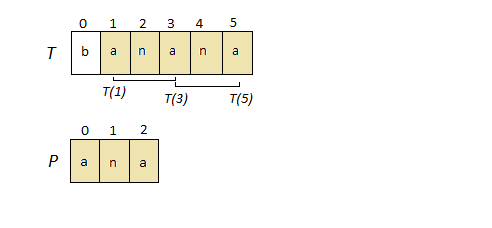
\includegraphics[width=0.4\textwidth]{1}
    \captionsetup{width=0.8\textwidth}
    \caption{The text $T$=\{banana\} and pattern $P$=\{ana\} over the alphabet $\Sigma$=\{abn\}. The pattern $P$ occours in $T$ in, at position $T[1]$ and $T[3]$. Notice that occurrences of $P$ may overlap.}
    \label{fig:banana}
\end{figure}
\newline
\\ 
Since most discussions of the exact string matching paradigm, begins with a naive method, this paper adobt the tradition, both presented by Gusfield et. al and by many others \cite{gusfield}. The naive method forms a basic understandig and insight to the more complex exact string mathing algorithms presented in the paper. 
\newline
The method align left end of $P$ with left end of $T$ and the scan from left to right, comparing characters of $P$ in $T$, until either there is a mismatch or $P$ is exhausted, in which case an occurence of $P$ in $T$ is reported. $P$ is then shifted one place to the right, and the character comparison is restarted from the left end of $P$ which repeats until $P$ shifts past right end of $T$ \cite{gusfield}.
\newline
Let $n$ denote the length of $P$ and let $m$ denote the length of $T$, then the worst-case timecomplexity of the naive method, is $\Theta$(nm). This is particular clear if $P$ and $T$ consists of the same repeated characters, such that the is an occurence of $P$ in $T$ for each of the first $m - n - 1$ positions.
\newline
Since most discussions of the exact string matching problem begin with the naive method. This paper adopt this tradition, as it form a basic insight to the more complex exact string matching algorithms presented later on \cite{gusfield}.
\begin{figure}[H]
    \centering
    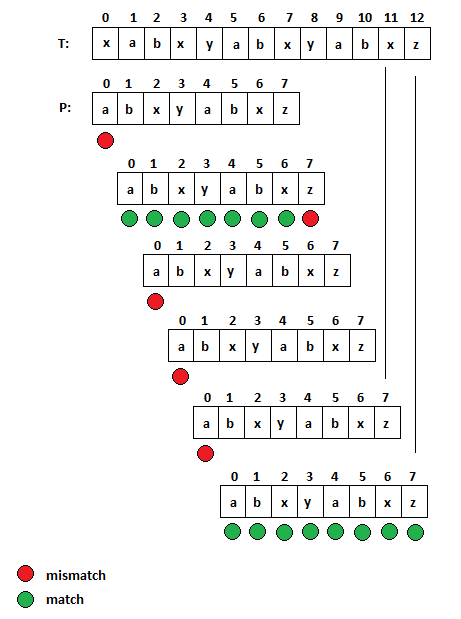
\includegraphics[width=0.4\textwidth]{comparisonbased1}
    \captionsetup{width=0.8\textwidth}
    \caption{The naive method, where $P$ is shifted one character to the right after each mismatch.}
    \label{fig:comparisonbased1}
\end{figure}

Let pattern $P$=  abxyabxz and let text $T$= xabxyabxyabxz.
\\ \\
Then the naïve method align left end of $P$  with left end of $T$ and scan from left to right, comparing the characters of $P$ with $T$, until either two disparate characters are located or $P$ is exhausted, in which case an occurrence of $P$ in $T$ is reported. If a character mismatch happens, $P$ is shifted one place to the right, until $P$ exceeds $T$, as illustrated in Figure \ref{fig:comparisonbased1} \cite{gusfield}.
The worst-case bound of the naïve method is $\Omega$(nm), which can be reduced to $\Omega$(n + m) with the basic idea of shifting $P$ more than one character at a time. This means that the number of character comparisons are reduced, due to $P$ moving through $T$ more rapidly. Some methods even exploit skipping over parts of the pattern after $P$ has shifted, further reducing character comparisons \cite{gusfield}. 
\begin{figure}[H]
    \centering
    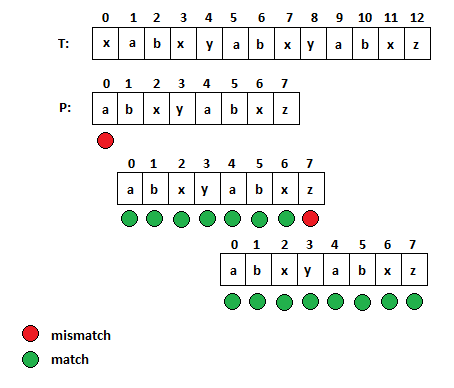
\includegraphics[width=0.4\textwidth]{comparisonbased2}
    \captionsetup{width=0.8\textwidth}
    \caption{After a mismatch, $P$ is shifted to the next occurrence of $a$ at position 5 in $T$, moving through $T$ more rapidly}
    \label{fig:comparisonbased2}
\end{figure}
\newline   
Figure \ref{fig:comparisonbased2}  illustrates the idea of shifting $P$ more than one character to the right. At initialization , the left end of $P$ aligns with left end of $T$, here comparing each character from $P$ with $T$ from left to right.
\newline
Let $P[0]$ denote the starting character of $P$ found at position 0, such that $P[0]=a$
\newline
\begin{figure}[H]
    \centering
    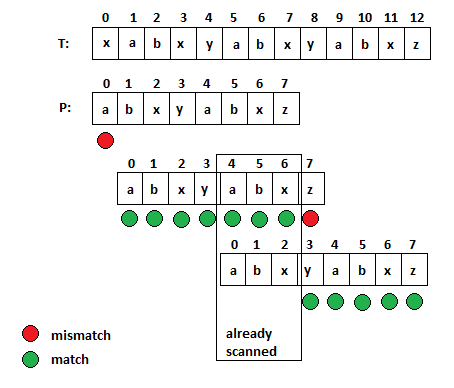
\includegraphics[width=0.4\textwidth]{comparisonbased3}
    \captionsetup{width=0.8\textwidth}
    \caption{Characters that have already been scanned are stored, so when $P$ is shifted to position 5 in $T$, $abx$ have already been scanned and can be skipped, and the character scanning is resumed from position 8 and 3, in $P$ and $T$, respectively.}
    \label{fig:comparisonbased3}
\end{figure}
When comparing characters, if a character in $T$ match $P[0]$, store the location. If a mismatch occur, shift $P$ to the stored location, here position 5 in $T$ and restart the character comparison, as in Figure \ref{fig:comparisonbased2}. This is doable for the reason that $P[0]=a$ does not occur in $T$ before position 5, such that $T[5]=P[0]=a$. 
The method in Figure \ref{fig:comparisonbased2} can be improved further, knowing that the next  three  characters are $abx$ after $P$ has shifted to position 5 in $T$. Knowing this, the first three characters are skipped, and character scanning are resumed from position 8 in $T$ and position 3 in $P$, as illustrated in Figure \ref{fig:comparisonbased3} \cite{gusfield}. 
\newline
The three methods presented exemplifies the basic idea of comparison based algorithms. More efficient algorithms have been developed, such as the Boyer-Moore and Knuth-Morris-Pratt algorithm, which have been implemented to run in linear time $(O(n+m) time)$ \cite{gusfield}. These are without a doubt interesting algorithms to analyze, however this paper merely delivers a short and precise description of the paradigm.
Another approach to the comparison based method is the preprocessing approach, where comparisons are skipped by first spending a small amount of time, learning about the internal structure of pattern $P$ or text $T$. Some methods preprocess pattern $P$ to solve the exact string matching problem, where the opposite approach is to preprocess text $T$, such as algorithms based on suffix trees \cite{gusfield}.

\subsection{Suffix trees}

The classic application for suffix tree is the substring problem \cite{gusfield, Kunihiko}, which is both a data structure -and an algorithmic problem \cite{mit}. That is, given a long text $T$ over some alphabet $\Sigma$, and some pattern $P$, the substring problem consist of preprocessing $T$ in linear time $O(m)$, and hereafter  $T$ should be able to take any unknown pattern $P$, and in linear time $O(n)$ determine occurrences of $ P$, if any, in $T$ \cite{gusfield}. The preprocessing time is here proportional to the length of text $T$, and the query is proportional to the length of pattern $P$ \cite{gusfield}. 
\newline
This paper adopts the approach of Gusfield et al., by not applying the denotation of pattern $P$ and text $T$, in respect to describing suffix trees. By using the general description and denotation of suffix trees, there will be less confusion, since input string can take different roles and vary for application to application \cite{gusfield}.
\newline
\newline
Conceptually a suffix tree is a compressed trie \cite{mit}.  
\begin{quote}
\textbf{Definition}    A trie contains all suffixes of string $S$, where each edge is labeled with a character from some alphabet $\Sigma$. Each path from root to leaf represent a suffix, and every suffix is represented with some path from root to leaf \cite{mit,Kunihiko}.
\end{quote}
\begin{figure}[h]
    \centering
    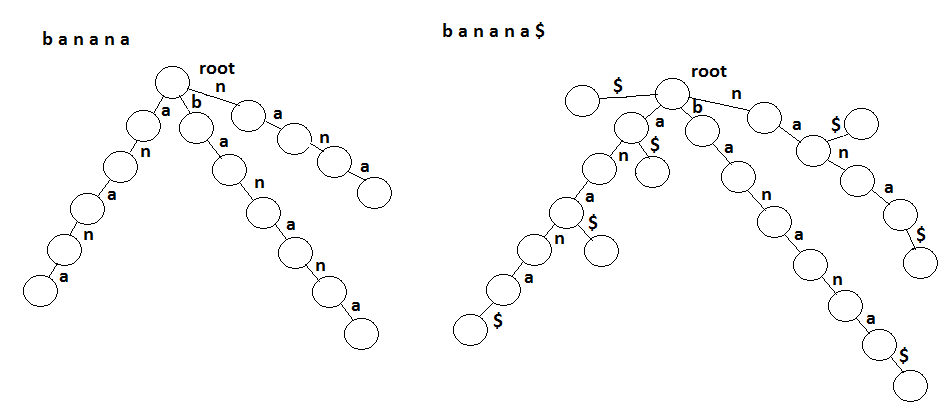
\includegraphics[width=0.6\textwidth]{trie}
    \captionsetup{width=0.8\textwidth}
    \caption{Left is a trie of the string $banana$ and the right is a trie of the string $banana\$$.}
    \label{fig:trie}
\end{figure}
\newline
Figure \ref{fig:trie} illustrates two tries, left of the string banana and the right over the string $banana\$$. Note that right trie has the termination character $\$$ appended to the end. This is due to the fact that the definition of a trie dictates that every suffix is represented with some path from root to leaf. Suffix $ana$ in left trie does not have a path from root to leaf, but appending a termination character to S that exists nowhere else in the string, will eliminate the problem.
\newline
Creating a compressed trie, one takes each non-branching nodes and compress them, such that edge-labels from non-branching nodes concatenates into a new edge-label, as illustrated in Figure \ref{fig:comprestrie}. Here node 1 is a non-branching node, one then concatenate a to n, to form a new edge-label na, deleting the non-branching node \cite{mit}. The number of non-branching nodes in a trie is at most the number of leaves. By compressing, we know have that the number of internal nodes is at most the number of leaves, having O(k) nodes total.
\newline

\begin{figure}[h]
    \centering
    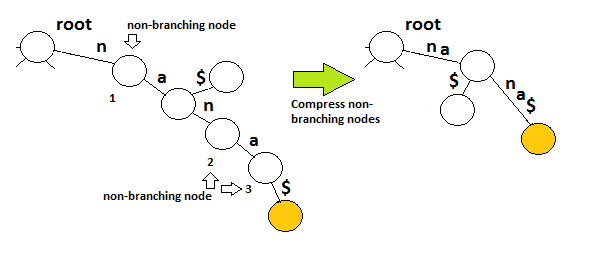
\includegraphics[width=0.6\textwidth]{compressingtrie}
    \captionsetup{width=0.8\textwidth}
    \caption{Compressing a trie.}
    \label{fig:comprestrie}
\end{figure}
\begin{quote}
\textbf{Definition}   A Suffix tree, $T$, is a $m$-character string $S$ concatenated with a termination character $\$$, that is represented as a directed rooted tree with exactly $m$ leaves, numbered $1$ to $m$. Except the root, each internal node contains at least two children, with each edge labeled with a nonempty substring of S. No two edges exiting a node can have labels beginning with the same character. The concatenation of edge-labels on the path from the root to leaf i, unerringly spells out the suffix of $S$ that starts at position i, such that it spells out $S[i..m]$. The termination character $\$$ is assumed to appear nowhere else in $S$, such that no suffix of the consequential string can be a prefix of any other suffix\cite{gusfield}.
\end{quote}
\begin{figure}[h]
    \centering
    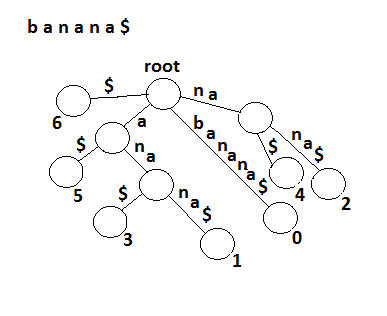
\includegraphics[width=0.4\textwidth]{suffixtree(banana)}
    \captionsetup{width=0.8\textwidth}
    \caption{A suffix tree $T$ for string $banana\$$.}
    \label{fig:suffixTree}
\end{figure}
The suffix tree for the string $banana\$$, in lexicographical order, is illustrated \ref{fig:suffixTree}. Each path from the root to a leaf $i$, unerringly spells out a suffix of $S$, starting at position $i$ in $S$. As an example, leaf numbered $2$ spells out $nana\$$, starting at position $2$ in the $S$, such that $S[2..6] = nana\$$. Each node has at least two children, and no two edges exiting a node begins with the same character. 
\newline
To dive into the substring problem using linear preprocessing time, $O(m)$, and linear search time, $O(n)$ we follow the tradition, and starts with a naive and straightforward algorithm to building suffix trees before verturing into the linear time preprocessing approach \cite{gusfield}. 


\subsection{Suffix Trees To Suffix Arrays In Linear Time}

Firsrt, suppose we used a suffix tree as datastructure for an application that resign on a device with abundance of space, but needed it to run a smaller device where the current datastructure would be too large. Then we could convert the suffix tree to the space efficient suffix array, provided that the current operations on the suffix tree is supported by the suffix array \cite{gusfield}. 
\\ \\
\textbf{Deffinition}
\begin{quote}
 Let an $edge(v, u)$ in $T$ be lexically less than an $edge(v, w)$ if, and only if the first character in $edge(u, v)$ is lexically less than the first character in $edge(v, w)$ \cite{gusfield}
\end{quote}
\\
As no two edges out of $v$ have labels beginning with the same character, edges out of $v$ lexical ordered. So the path from the root of $T$ following the lexically smallet edge out of each node leads to a leaf in $T$ which represents the lexically smallet suffix in $T$. Then the suffix array $SA$ of $T$ can be constructed in linear time.
For suffix tree $T$= banana in Figure \ref{fig:suffixTree}, the lexical depth-first traversal visites the nodes 6, 5, 3, 1, 0, 4, 2 in that order \cite{gusfield}. 
\\
Latter, suppose that we have no datastructure constructed for our new application, but already know that a suffix tree would be too large for our new device. Then it would be easier if we could construct the suffix array without the need of a pre-constructed suffix tree, especially if we could construct it in linear time. Luckily we can, but besides of being more space effecient a more detailed description is needed.

\subsection{Suffix Arrays} \label{Suffix Arrays Section}

Suffix array are space efficient alternatives to suffix trees \cite{gusfield,twoeffecient}. Before Manber and Meyers in 1990 introduced the first direct suffix array construction algorithm – SACA, suffix arrays were constructed using lexicographical-order traversal of suffix trees  \cite{gusfield,twoeffecient, performancesuffix, newapproach}. Manber and Meyers made suffix trees obsolete in respect to constructing suffix arrays, and their approach is known as a doubling algorithm, where with each sorting pass, doubles the depth to which each suffix are sorted. This means that suffixes are sorted in logarithmic number of passes, providing a worst case bound of $O(n log n)$ and $O(n)$ expected, assuming linear sort, reminiscent of Radix Sort \cite{performancesuffix} and queries can be answered in $O(P + log n)$ with use of Binary Search \cite{gusfield}.
\\
With the discovery of four different SACAs requiring only $O-(n)$ time worst case in 2003, the situation drastically changed. SACAs have since been the focus of intense research \cite{performancesuffix,newapproach}. In 2005 Joong Chae Na introduced more linear time SACAs, where two stood out, the Ko-Aluru (KA) algorithm for supplying good performance in practice and the Kärkkäinen-Sanders algorithm for its elegance \cite{newapproach}. 
\\
According to a survey paper, SACAs have to fulfill three important requirements: 
\begin{quote}
1. The algorithm should run in asymptotic minimal worst case time, where linear is an optimal way \cite{newapproach}. 
\end{quote}
\begin{quote}
2. The algorithm should run fast in practice \cite{newapproach}.
\end{quote}
\begin{quote}
3. The algorithm should consume as less extra space in addition to the text and suffix array as possible, where constant amount is optimal \cite{newapproach}.
\end{quote}
Although no current SACAs fulfill the requirements in an optimal way, research into faster and more space reducing SACAs continued \cite{newapproach}. Later on, in 2009, Nong et al. introduced two new linear time construction algorithms, one which outperformed most known and existing SACAs, called Suffix Array Induced Sorting SA-IS algorithm, guaranteeing asymptotic linear time and almost optimal space requirements \cite{newapproach}. 


\subsection{SAIS - Suffix Array Induced Sorting Algorithm} \label{SAIS Section}

The SA-IS algorithm  is a divide and conquer and recursion algorithm, using variable-length leftmost S-type substrings and induced sorting \cite{twoeffecient}. In view of the fact that the SA-IS algorithm is unsophisticated to comprehend, implement and guarantees asymptotic linear time construction and close to optimal space,  SA-IS has been chosen as the single algorithm for the implementation of a malware detection system and the experiments which follow. 

\begin{quote}
\begin{lstlisting}[ basicstyle=\scriptsize, %or \small or \footnotesize etc.
]
SAIS(S, SA)
    (* Step 1 : Initialization & classification*)
    SA <-- suffix array of S
    t <-- type array
    P <-- LMS indicies array
    B <-- bucket array
    Scan S once from either left or right and classify all characters as 
        S-type or L-type and place them in t.
    Scan t once from  either left or right and locate all LMS substrings 
        in S and put them into P_1
    (* Step 2 : Induced sort LMS-substring)
    Induced sort all LMS substrings using P_1 and B
    Name each LMS substring in S by its bucket index to get a 
        new shortened string S_1
    (* Step 3 : Uniqueness - recursive step)
    (*@\textbf{if}  @*) T_1 is distinct, hence all characters are unique
       (*@\textbf{then}  @*) 
           Directly compute SA_1 from S_1
       (*@\textbf{else}  @*) 
           SAIS(S_1, SA_1)
    (* Step 4 : Induce SA from SA_1)
    Induce SA from SA_1       
    (*@\textbf{return}  @*) 
\end{lstlisting}
\end{quote}

\textbf{Basic notations}
\\ \\
Let $S$ be a string or text of $n$-characters stored in an array $[0…n-1]$ and let $\Sigma(s)$ be the alphabet of $S$. 
\\ \\
Let $S$$\$$ be a string $S$ concatenated with the termination symbol $\$$, where $\$$ is not contained in $S$ and is the lexicographical smallest character in $S$. For $S$ containing concatenation of multiple strings, let $S={S_0\$S_1\$...S_{n-1}\$}$, where $\$$ is the termination symbol for each concatenated string in $S$, and is the lexicographical smallest character in $S_0,S_1,...,S_{n-1}$. Furthermore, $S$ may not be contained in $S_0,S_1,...,S_{n-1}$. String $S$ is supposed to be concatenated with the unique termination symbol $\$$, if not explicit   stated otherwise \cite{twoeffecient}.
\\ \\
Let $suf(S,i)$ be some suffix in $S$ starting at $S[i]$ running to the termination symbol $\$$. $suf(S,i)$ is of S-type or L-type if $suf(S,i) < suf(S,i+1)$ or $suf(S,i) > suf(S,i+1)$, respectively \cite{twoeffecient}.
\\ \\
Let $suf(S, n-1)$ be the termination symbol and of S-type \cite{twoeffecient}.
\\ \\
Let $S[i]$ be S-type or L-type, if suf(S,i) is S-type or L-type, respectively \cite{twoeffecient}.
\\ \\
\textbf{Observation}
\begin{itemize}
  \item $S[i]$ is  S-type if $S[i] < S[i+1]$ or $S[i] = S[i+1]$ and $suf(S, i+1)$ is S-type \cite{twoeffecient}.
  \item $S[i]$ is  L-type if $S[i] < S[i+1]$ or $S[i] = S[i+1]$ and $suf(S, i+1)$ is L-type \cite{twoeffecient}.
\end{itemize}

The properties defined in the observation suggest that scanning from right to left, determing the type of each suffix or character can be done in constant time, $O(1)$, and that the type array $t$, can be filled in linear time, $O(n)$ \cite{twoeffecient}.

\begin{figure}[H]
    \centering
    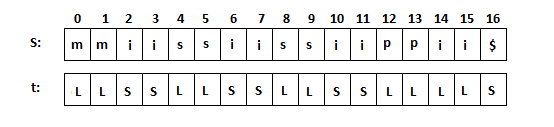
\includegraphics[width=0.6\textwidth]{SAISmmii1}
    \captionsetup{width=0.8\textwidth}
    \caption{Type array $t$ is filled from right to left}
    \label{fig:SAISmmii1}
\end{figure}

Figure \ref{fig:SAISmmii1} illustrates the filled type array, $t$, for text $S$=mmiissiissiippii\$, where text $S$ is scanned from right to left, determining the type of each suffix and character. Going from right to left in Figure \ref{fig:SAISmmii1} we have that $suf(S,16)$=\$ is a S-type, $suf(S,15)$=i\$ > $suf(S,16)$=\$ and is L-type, $suf(S,14)$=ii\$ > $suf(S,16)$=i\$ and is L-type and so forth, filling the type array $t$ in linear time.
\\ \\
Let $S[i]$ be a left most S-typeLMS character, if $S[i]$ is S-type and $S[i-1]$ is L-type, and let $suf(S,i)$ be a LMS suffix, if S[i] is a LMS character \cite{twoeffecient}.
\\ \\
Let $S[i..j]$ be a LMS substring if both S[i] and S[j] are LMS characters, and there exists no other LMS characters in the substring, and $i \neq j$ or it is the sentinel itself \cite{twoeffecient}.
\\ \\

\begin{figure}[H]
    \centering
    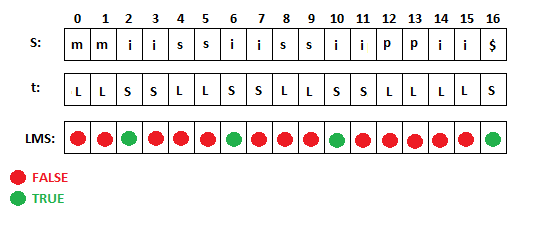
\includegraphics[width=0.6\textwidth]{SAISmmii2}
    \captionsetup{width=0.8\textwidth}
    \caption{Type array $t$ and LMS array defined for S=mmiissiissiippii\$}
    \label{fig:SAISmmii2}
\end{figure}

As Figure \ref{fig:SAISmmii2} exemplify, four LMS characters are defined for $S$=mmiissiissiippii\$, here at position 2, 6, 10 and 16 in $S$. Furthermore, four substrings and suffixes exists in $S$, namely $S[2..6]$, $S[6..10]$, S[10..16] and S[16..16], and $S[2..16]$, $S[6..16]$, S[10..16] and S[16..16], respectively.
After defining the S-types, L-types and LMS, the induction process of LMS substrings commence.
\\ \\

\textbf{Deffinition}
\begin{quote}
Determining the order of any two substrings, the corresponding characters are compared from left to right, comparing their lexicographical values first, and next their types, where S-type is considered highter priority than L-type \cite{twoeffecient}.
\end{quote}

\textbf{Induced sorting LMS substrings}
\\ \\
This part address the challenging problem of sorting the variable length LMS substrings. The basic idea is to create a new array, SA, and bucket sort the LMS substring into their equivalent buckets. Each bucket is named corresponding to the alphabet $\Sigma=\{\$,i,m,p,s\}$ in lexicographical order, such that SA contains four buckets, named $\$$, $i$, $p$ and $s$ in that order, as shown in Figure \ref{fig:SAIS_LMS} \cite{twoeffecient}.
$S$ is scanned from left to right, and indices for each LMS substring is appended to the end of its corresponding bucket in $SA$. The first LMS substring index is placed at the end of bucket for $i$, here at position 8 in $SA$ and forwards the bucket end one to the left, hence the bucket end for $i$ now rest at position 7 in $SA$. This process is repeated until all LMS substring indicies are placed in their buckets \cite{twoeffecient}.

\begin{figure}[H]
    \centering
    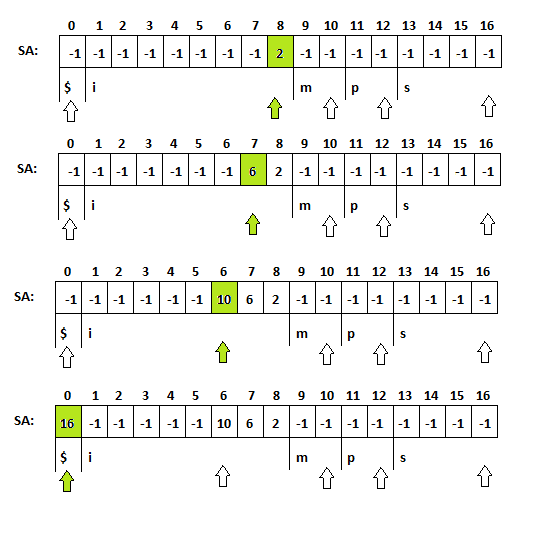
\includegraphics[width=0.5\textwidth]{SAIS_LMS}
    \captionsetup{width=0.8\textwidth}
    \caption{Induced sort of LMS substring}
    \label{fig:SAIS_LMS}
\end{figure}

When the LMS substrings are placed, then scan $SA$ from left to right and for each nonnegative value $S[i]$, if $S[i]-1$ is L-type, then place $SA[i]-1$ in the corresponding bucket for $suf(S, SA[i]-1)$, and lastly forward the bucket head one to the right \cite{twoeffecient}. 
\begin{figure}[H]
    \centering
    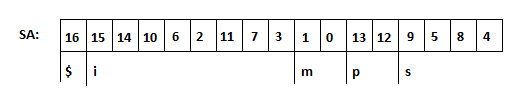
\includegraphics[width=0.5\textwidth]{SAIS_LMSfinal}
    \captionsetup{width=0.8\textwidth}
    \caption{$SA$ after the induced sorting for LMS substring.}
    \label{fig:SAIS_LMSfinal}
    
\end{figure}
\\
Roughly equivalent, when all L-types are placed, scan $SA$ from right to the left for each nonnegative value S[i], if $S[i]-1$ is S-type, then place $SA[i]-1$ in the corresponding bucket for $suf(S, SA[i]-1)$, and forward the bucket end one to the left. The above operations are demonstrated in Appendix \ref{SAIS Algorithm run} and the final result is displayed in Figure \ref{fig:SAIS_LMSfinal} \cite{twoeffecient}.
\\ \\
It is now the matter of determine if all LMS substrings are correctly sorted in SA, hence the uniqueness step in the SAIS algorithm. This is done by scanning $SA$ from left to right, and obtaining each LMS substring, and comparing the lexicographical values and types, and place them in buckets named accordingly to the lexicographical order they appear, starting from 0. So scanning from left to right in $SA$ given in Figure \ref{fig:SAIS_LMSfinal} gives the following bucket $B = \{\{0; \$\}, \{1; iippii\$\}, \{2; iissi, iissi\}\}$. The bucket keys are then placed in $S_1$ in the order as they appear in the original string $S$, hence $S_1 = \{2,2,0,1\}$ as illustrated in Figure \ref{fig:SAIS_LMSS}. If each character in $S_1$ is unique, hence does not exists any where else in $S$, then $SA_1$ can be computed directly from $S_1$, else fire the recursive step $SAIS(S_1, SA_1)$. $S_1$ for $S$ in Figure \ref{fig:SAIS_LMSS} is not distinct, since $2$ exists twice in $S_1$, hence $2$ is not unique, consequently a recursive step, $SA(S_1, SA_1)$,  is needed. Before venturing into the recursive step, save the original positions of the LMS substrings as they appear in $S_1$ into $P_1$, where $S_{1}[0] = 2$ points at position 2 in $S$,  $S_{1}[1] = 2$ points at position 6 in $S$, $S_{1}[2] = 1$ points at position 10 in $S$ and finally $S_{1}[3] = 0$ points at position 16 in $S$, such that $P_1=[2; 6; 10; 16]$ \cite{twoeffecient}.
\\
\begin{figure}[H]
    \centering
    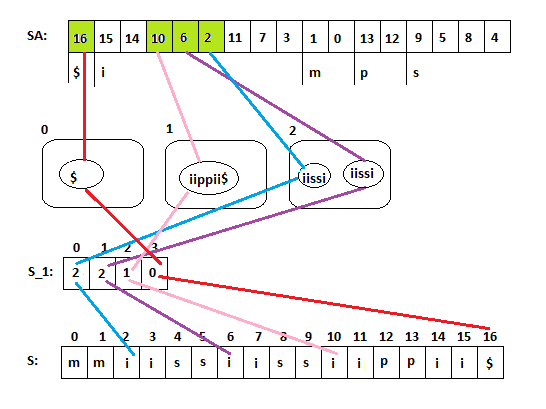
\includegraphics[width=0.5\textwidth]{SAIS_LMSS}
    \captionsetup{width=0.8\textwidth}
    \caption{Building $S_1$ from $SA$, using the original positions of the LMS substrings in $S$.}
    \label{fig:SAIS_LMSS}
\end{figure}
\\
In the recursive step for $SAIS(S_1, SA_1)$, locate S-types, L-types and LMS characters/substrings and determine if $S_1$ is distinct. In this case, as demonstrated in Figure  \ref{fig:SAIS_RECURSIVE}, there is only one LMS substring in $S$ so the new string $S_1$ is trivially distinct.
\\ \\
\textbf{Induce sort $SA$ from $SA_{1}$}
\\ \\
Either $SA_{1}$ has been computed directly from $S$ (if $S$ is distinct) or returned from one or more recursive steps. In either case, $SA$ can be induced sorted from $SA_1$ using information bound in $P_1$ \cite{twoeffecient}. 
\\ \\
First initialize all indicies in $SA$ with $-1$ and find the bucket ends. Then scan $SA_1$ from right to left and place $P_1[SA_1[i]]$ at the corresponding bucket end, and forward the bucket end one item to the left \cite{twoeffecient}. 
 \\
Then sort L-types by scanning $SA$ from left to right for each non-negative item $SA[i]$. If  $SA[i-1]$ is L-type, place $SA[i-1]$ in the corresponding bucket head for $SA$ and forward the bucket head one item to the right \cite{twoeffecient}.
\\
Last, sort all S-types by scanning SA from right to left for each non-negative item SA[i]. If  $SA[i-1]$ is S-type, place $SA[i-1]$ in the corresponding bucket end, and forward the bucket end one item to the left \cite{twoeffecient}. 
\\
\begin{figure}[H]
    \centering
    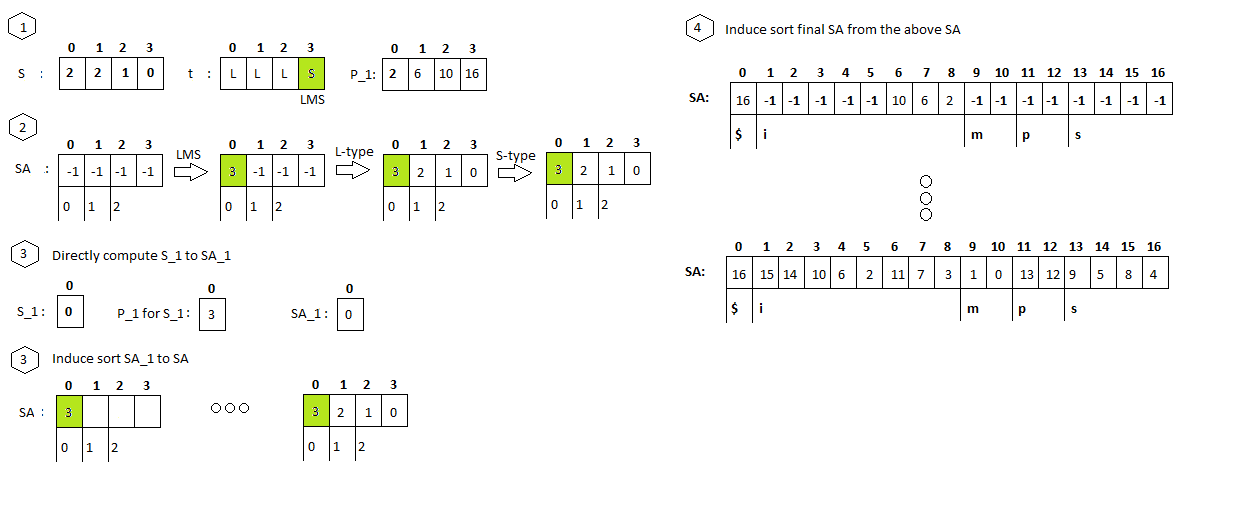
\includegraphics[width=1.0\textwidth]{SAIS_RECURSIVE}
    \captionsetup{width=0.8\textwidth}
    \caption{The recursive step $SA(S_1, SA_1)$.  First S-types, L-types and LMS characters/substrings for $S_1$ is localized. Secondly, induced sort LMS substrings, such that $SA_1 = [3;2;1;0]$. Last, scan $SA_1$ from right to left and place $P_1[SA_1[i]]$ into the buckets end of $SA$ as described for induced sorting LMS Substrings, for each item in $SA_1$. The final result is displayed in step 4.}
    \label{fig:SAIS_RECURSIVE}
    
\end{figure}
\\
This procedure is demonstrated in Figure \ref{fig:SAIS_RECURSIVEDESCRIPTION} where $SA$ is induced sorted from $S$ for the text $T$=mmiissiissiippii\$. SAIS returns the suffix array $SA$=[16; 15; 14; 10; 6; 2; 11; 7; 3; 1; 0; 13; 12; 9; 5; 8; 4] for text $T$=mmiissiissiippii\$ which is indeed sorted in lexicographical order as illustrated in Figure \ref{fig:SAIS_Sortedorder} \cite{twoeffecient}.
\\
\begin{figure}[H]
    \centering
    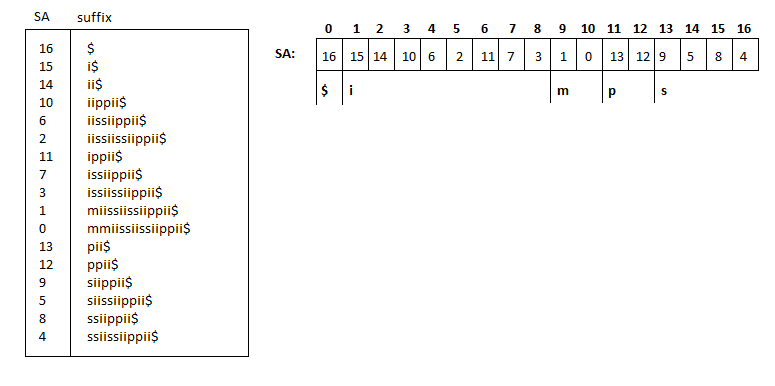
\includegraphics[width=0.6\textwidth]{SAIS_Sortedorder}
    \captionsetup{width=0.8\textwidth}
    \caption{The suffix array for the text $T$=mmiissiissiippii\$.}
    \label{fig:SAIS_Sortedorder}  
\end{figure}
\\ \\
\textbf{Correctness, completeness and performance}
\\ \\
We shown a thorough run-through of the SA-IS algorithm, now we tend to correctness, completeness and the performance. We claimed that SAIS is a linear time suffix array construction algorithm using divide-and-conquer and recursion techniques. Furthermore we claimed that the consequential constructed suffix array contains indices of all suffixes of a legal input $S$ according to their lexicographical order. Ge Nong et al. \cite{twoeffecient} already proved these attributes of SA-IS, we merely elaborate with examples. Recall that $S$ must be terminated with the sentinel and of such, is not a legal input, if $S$ is not terminated by the sentinel. Furthermore, the sentinel must be the unique smallest character in $S$, and exist nowhere else in $S$.  
\\ \\
\textit{Induced Sorting LMS-Substrings \& Inducing $SA$ from $S_1$ }
\\ \\
Step two and three in both induced sorting LMS-substring and inducing $SA$ from $S_1$ are equivalent. In induced sorting LMS-substrings we scan S from right to left and append LMS indices in their correspobding buckets in $SA$ and in inducing $SA$ from $S_1$, $S_1$ is scanned from right to left and we append $P_1[SA_1[i]]$ into their corresponding bucket's in $SA$.
The sorting of the variable-size LMS-substrings is the most challenging problem. Ge Nong et al. \cite{twoeffecient} solves the problem by induced sorting. We have earlier shown this procedure with an example for $S$=mmiissiissiippii\$ and will continue down this road to elaborate the proof presented by Ge Nong et al. \cite{twoeffecient}.
\begin{quote}
\textbf{Theorem 4.4} Induced sorting LMS substrings will correctly sort all LMS prefixes of $S$ into $SA$. \cite{twoeffecient}.
\end{quote}
First, let LMS prefix $pre(S, i)$ of $suf(S, i)$ to be either the sentinel itself when $i = n-1$ or prefix $S[i..k]$ in $suf(S, i)$ where $i \neq n-1$, $k > i$ and $S[k]$ is the first LMS character after $S[i]$. LMS prefix $pre(S,i)$ is defined as L-type of S-type if $suf(S, i)$ is L-type or S-type \cite{twoeffecient}.
\\ \\
Then suf(S,5) is L-type, hence pre(S, 5) is L-type and pre(S, 5)=$S[i \ldots k] = S[5 \ldots 6]$ = si, since $S[k=6]=i$ is the first LMS character after $S[i]$. 
\\ \\
\begin{figure}[H]
    \centering
    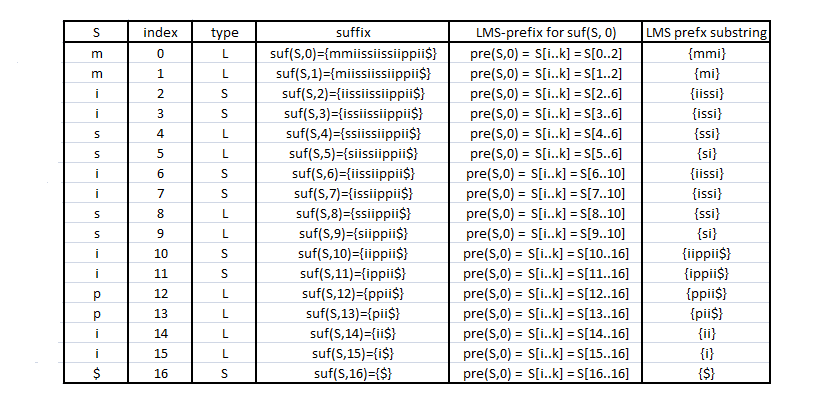
\includegraphics[width=0.8\textwidth]{lmsprefix}
    \captionsetup{width=0.8\textwidth}
    \caption{Suffixes with corresponding LMS prefixes $T$=mmiissiissiippii\$.}
    \label{fig:lmsprefix}  
\end{figure}
Suppose we appended all LMS-substring indices in $SA$ for $S$=caa\$ with the following L-types and S-types illustrated in Figure \ref{fig:ltypedescription}. Then for each non-negative item in $SA$ we encounter when scanning from left to right, we ask if suf(S, i) has an immediate left neighbor suf(S, i-1) that is lexicographical larger than suf(S, i) and therefore should be appended to the right of suf(S, i) in $SA$. As illustrated in Figure \ref{fig:ltypedescription}, each immediate left neighbor suf(S, i-1) in $S$ scanning from right to left in $S$ is lexicographical larger than suf(S, i). The only LMS-character in $S$ is $S[3]$=\$, the sentinel itself, and its immediate left neighbor is of L-type, and should be appended to its appropriate bucket head, and the head is forwarded one item to the right. Next non-negative item we encounter in $SA$ is suf(S, 2), it immediate left neighbor suf(S,1) is of L-type and is therefore lexicographical larger than suf(S, i), so it should be added to the right of suf(S,i). Since S[1]=a, suf(S,1) should be appended in the bucket head for $a$, but should also be to the right of suf(S,2) which is already in bucket $a$ in $SA$. Luckily we forwarded the bucket's head one item to the right, thus suf(S,1) will be appended after suf(S, 2) in $SA$. This entails that any immedite left neighbor $SA[i-1]$ of $SA[i]$, $suf(S, SA[i-1])$ is lexicograpical larger than $suf(S, SA[i])$.
\begin{figure}[H]
    \centering
    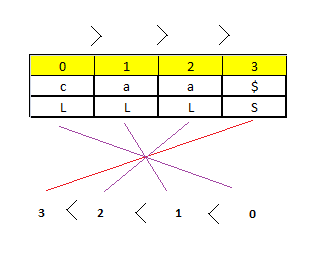
\includegraphics[width=0.4\textwidth]{ltypedescription}
    \captionsetup{width=0.8\textwidth}
    \caption{L-types and S-types for $S$=caa\$, where $S[0 \dots 3] > S[1 \dots 3] > S[2 \dots 3] > S[3 \dots 3]$.}
    \label{fig:ltypedescription}  
\end{figure}
When inserting L-type pre(S,i) of suf(S,i) in $SA$, we must ensure that each L-type $pre(S,i)$ for $suf(S,i)$ is sorted correctly for all S-type $pre(S,i)$ of $suf(S,i)$ in $SA$ \cite{twoeffecient}. Figure \ref{fig:lmsprefix} illustrate suffixes and LMS-prefixes for $S=mmiissiissiippii\$$. Suppose that $k$ number of L-type LMS-prefixes are correctly sorted into SA and suppose that we append the ($k$+1)th L-type LMS-prefix $pre(S,i)$ to the head of its corresponding bucket and there is already a greater $pre(S,j)$ in front of $pre(S,i)$, e.g. to the left of $pre(S,i)$. This consequently signify that character $S[i]=S[j]$ since they are in the same bucket, $pre(S, j+1) > pre(S, i+1)$ and $pre(S, j+1)$ is in front of $pre(S, i+1)$. If this is the case, we must have scanned SA from the left to the right, and discovered LMS-prefixes that are not sorted correctly. This is a contradiction and imply that all L-type LMS-prefixes are sorted in correct order in $SA$ \cite{twoeffecient}. 

In the last step we append S-type LMS-prefixes and consequently sort all LMS-prefixes in $SA$. We scan $SA$ from right to left, and for each non-negative index $i$, if suf(S,i-1) is of S-type, append it to the bucket end of its corresponding bucket, and forward the bucket end one to the left. \\
In similar manner to the prove of L-type, by contradiction, suppose that $k$ S-type LMS-prefixes are appended to their corresponding bucket ends and sorted correctly. Suppose that when we append the $k+1$th LMS-prefix pre(S, i) to its corresponding bucket end there is already a smaller S-type LMS-prefix pre(S, j) behind pre(S, i), e.g. to its right. This must entail that S[i] = S[j], since they are in the same bucket, pre(S, j+1) < pre(S, i+1), and pre(S, j+1) is behind pre(S, i+1) in $S$. This implies that when $SA$ where scanned from right to left, before adding pre(S, i) to its bucket, we must have stumbled by LMS-prefixes in $SA$ that were not sorted correctly \cite{twoeffecient}.
\begin{figure}[H]
    \centering
    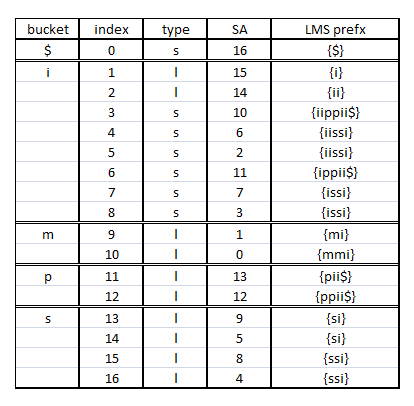
\includegraphics[width=0.5\textwidth]{lmssorteds}
    \captionsetup{width=0.8\textwidth}
    \caption{Sorted S-type LMS-prefixes of  $T$=mmiissiissiippii\$.}
    \label{fig:lmssorteds}  
\end{figure}

When appending S-type LMS-prefixes to their equivalent buckets, we may overwrite already appended S-type LMS-prefixes. Figure \ref{fig:lmssorteds} show the appended S-type LMS-prefixes and as proven, all LMS-prefixes are now sorted in $SA$ applying the same logic as with L-type LMS-prefixes \cite{twoeffecient}. We observe that every LMS-substring is a LMS-prefix, hence from the above proofs we can derive the following  properties. All LMS-substrings are as well LMS-prefixes, therefore sorting LMS-prefixes will thus  correctly sort all LMS-substrings. Furthermore, every substring in $S$ is a prefix of a LMS-prefix, hence sorting all LMS-prefixes will consequently sort every substring in $S$ \cite{twoeffecient}.
\\ \\
\textbf{Divide-and-conquer \& recursion}
\\ \\
As LMS-substrings are treated as basic blocks of the string in $S$, sorting all LMS-substrings will consequently sort all  substrings in $S$, as proven. Whenever two (or more) LMS-substrings is contained in the same bucket, we have a case where we have equal LMS-substrings. We then use the order index of each LMS-substring and replace LMS-substrings in $S$ with their names, as illustrated in \ref{fig:SAIS_LMSS}. $S$ can then be represented by a shorter string $S_1$, consequently solving the problem in a divide-and-conquer manner using recursion \cite{twoeffecient}. So we divide the problem into subproblems that are smaller instances of the original problem. Solve the subproblems recursively  and combine the solutions of the subproblems into a solution for the original problem \ref{introduction}.
Ge Nong et al. \cite{twoeffecient} proves that $||S_1||$ is at most $||S||$ eg. $n_1 \leq \lfloor n/2 \rfloor$, thus cutting the problem in half with each recursion, by sorting the LMS-substrings. In Figure \ref{fig:SAIS_RECURSIVE}, $S$=mmiissiissiippii\$ generated a shorter string $S$=3210. Here $||S_1||$ is at most half of $||S||$.
\\ \\
\textbf{Space and time complexity}
\\ \\
Ge Nong et al. \cite{twoeffecient} proves that all L-type or S-type suffixes of $S$ can be sorted in O(n) time, here with the knowledge that if all S-type suffixes have been sorted correctly in $SA$, all S-type andL-type suffixes can sorted in linear time by traversing $SA$ once from left to right \cite{twoeffecient}. Furthermore, knowing that the problem is reduced by at most half  $\lfloor n/2 \rfloor$at each recursion, we must have that:
\\ \\
T(n) = T($\lfloor n/2 \rfloor$) + O(n) = O(n)
\\ \\
Here the first O(n) counts for reducing the problem and inducing the final result from subproblem \cite{twoeffecient} and the last gives the result as an upper bound of O(n).
Space needed to store the sufix array for each reduced problem iteration is the akeelesheel for the space complexity. The first iteration is bound by $n \lceil log n \rceil$ bits, and descrease at most half for each iteration . This imply that the upper bound is governered by the first iterration and therefore the space complexity is O(n log n) bits \cite{twoeffecient}.

\subsection{Binary Search} \label{Binary Search Section}

\subsection{Longest Common Prefix - \empth{LCP}} \label{LCPsection}

The basic task of analysing a single genome, is to characterize and locate repeated elements of the genome. When comparring two or more genomes the task is to find similar subsequences of genomes. This makes repeat analysis to play a key role in the study, analysis and comparison of complete genome. 
A prefix in an definition for an affix placed before a word. Suppose we have $S$=abekat, then $abe$, $ab$ and $abek$ are prefixes, since they are an affixes placed before $kat$, $ekat$ and $at$, respectively. The longest common prefix amongst two string \emph{lcp($S_0, S_1$)} is the length of the longest word both strings share, from left to right. \\
Let $S_0$=abekat\$ and $S_1$=abe, then the longest common word is $abe$, hence lcp($S_0, S_1$)=3.

\subsection{Burrows-Wheeler Transform} \label{Burrows-Wheeler Transform}

The BWT - Burrow-Wheeler transform, invented by Burrow and Wheeler in 1994, also known as block sorting, is a lossless data compression algorithm and produces a permutation bwt(S) of an input string $S$, such that $S$ can be reversed from bwt(S), but is easier to compress \cite{BWT}. \\
BWT is a very powerful tool in data compression and even simple algorithms that implement BWT have good performance and achieve a good compression ratio using relative small space. Furthermore, even more powerful BWT-based compression tools, such as Bzip and Szip are still used today \cite{BWT}.
\\ \\
Besides data compression, BWT have a remarkable and practical property, namely that it can build a data structure which is sort of a compressed suffix array for a input string $S$ \cite{BWT}. To fully map and understand BWT, and how it succeed to create permutation bwt(S) of an input string $S$ that is easier to compress, this paper gives a precise description of the idea behind cyclic shifts and reversible lossless data compression, before venturing into property of building a data structure resembling compressed suffix array and its importance to the topic at hand. 
\\ \\
BWT consist of reversible transformation of input string $S$ denoted bwt(S). This reversible transformation, bwt(S), consist of exactly the same characters as in $S$ over same alphabet $\Sigma$, but is usually easier to compress. The idea is to form a conceptual matrix $M$ whose rows consist of cyclic shifts of $S$ sorted in a left to right lexicographical order \cite{BWT}.
\\ \\
Let $F$ denote the first column in $M$ and let $F_i$ denote the $i$-th character of column $F$. Almost equivalent, let $L$ denote the last column in $M$ and let $L_i$ denote the $i$-th character of column $L$ \cite{BWT}.
\\ \\
Then the following properties of $M$ can be defined:
\begin{itemize}
  \item Every column of $M$ is a permutation of $S$.
  \item For $i=2, \ldots , |2| + 1$, the character $L_i$ is followed by the character $F_i$ in $S$.
  \item Any character $\alpha$, the $i$-th occurrence of $\alpha$ in $F$ correspond to $i$-th occurrence of $\alpha$ in $L$. 
\end{itemize}

We assume that string $S$ is concatenated with the termination symbol $\$$. We first find each rotation of $S$ and place these in a matrix $M$, which can be done by repeatedly taking the end character of $S$ and sticking it to the front of $S$, until all rotations of $S$ is exhausted, as illustrated in Figure \ref{fig:Matrix0}. Then we sort the rows in lexicopgrapical order from top to buttom as in Figure \ref{fig:Matrix1} \cite{bwtfmindex}.

\begin{figure}[H]
\[
\begin{array}{*{11}c}
{\color{blue} F } &  &  & & & & & & & & {\color{red} L }  \\ 
{\color{blue} \$ } & a_0 & a_1 & a_2 & b_0 & b_1 & a_3 & a_4 & b_2 & a_5 & {\color{red} a_6 } \\
{\color{blue} a_6 } & \$ & a_0 & a_1 & a_2 & b_0 & b_1 & a_3 & a_4 & b_2 & {\color{red} a_5 }  \\
{\color{blue} a_5 } & a_6 & \$ & a_0 & a_1 & a_2 & b_0 & b_1 & a_3 & a_4 & {\color{red} b_2 } \\
{\color{blue} b_2  } & a_5 & a_6 & \$ & a_0 & a_1 & a_2 & b_0 & b_1 & a_3 & {\color{red} a_4 } \\
{\color{blue} a_4 }  & b_2 & a_5 & a_6 & \$ & a_0 & a_1 & a_2 & b_0 & b_1 & {\color{red} a_3 } \\
{\color{blue} a_3 }  & b_4 & b_2 & a_5 & a_6 & \$ & a_0 & a_1 & a_2 & b_0 & {\color{red} b_1 } \\
{\color{blue} b_1 }  & a_3 & b_4 & b_2 & a_5 & a_6 & \$ & a_0 & a_1 & a_2 & {\color{red} b_0 }  \\ 
{\color{blue} b_0 }  & b_1 & a_3 & b_4 & b_2 & a_5 & a_6 & \$ & a_0 & a_1 & {\color{red} a_2 } \\
{\color{blue} a_2 } & b_0 & b_1 & a_3 & b_4 & b_2 & a_5 & a_6 & \$ & a_0 & {\color{red} a_1 } \\
{\color{blue} a_1 } & a_2 & b_0 & b_1 & a_3 & b_4 & b_2 & a_5 & a_6 & \$ & {\color{red} a_0 }  \\
{\color{blue} a_0 } & a_1 & a_2 & b_0 & b_1 & a_3 & b_4 & b_2 & a_5 & a_6 & {\color{red} \$ } \\
\end{array}
\]
\captionsetup{width=0.8\textwidth}
\caption{Unsorted}
\label{fig:Matrix0}
\end{figure}

Then bwt(aaabbaabaa\$) = aab\$baaaaba, hence the string from $L$ in $M_{sorted}$ read from top to buttom. We notice that the characters tend to stick together in coloumn $L$. This feature is more obvious with longer strings. As an example, take string $S$=''tomorrow and tomorrow and tomorrow'', where bwt(''tomorrow and tomorrow and tomorrow'')= ''wwwdd  nnoooaatttmmmrrrrrooo  \$ooo'', if we were to compress this using run length encoding ($RLE$) we would get the shortened string ''3w2d2 2n3o2a3t3m5r3o2 \$3o'', hence we would have successfully compressed the original string using bwt(S) and RLE, such that RLE(bwt(S)) shortened the string from 34 to 23 characters, which is a reduction of appoximetly 26 \% \cite{bwtfmindex}. It is easy to see how one could reverse RLE compression back to bwt(S), but it is not obvious how one would reverse bwt(S) to the original string $S$ \cite{bwtfmindex}.

\begin{figure}[H]
\[
\begin{array}{*{11}c}
{\color{blue} F } &  &  & & & & & & & & {\color{red} L }  \\ 
{\color{blue} \$ } & a_0 & a_1 & a_2 & b_0 & b_1 & a_3 & a_4 & b_2 & a_5 & {\color{red} a_6 } \\
{\color{blue} a_6 } & \$ & a_0 & a_1 & a_2 & b_0 & b_1 & a_3 & a_4 & b_2 & {\color{red} a_5 }  \\
{\color{blue} a_5 } & a_6 & \$ & a_0 & a_1 & a_2 & b_0 & b_1 & a_3 & a_4 & {\color{red} b_2 } \\
{\color{blue} a_0 } & a_1 & a_2 & b_0 & b_1 & a_3 & b_4 & b_2 & a_5 & a_6 & {\color{red} \$ } \\
{\color{blue} a_3 }  & b_4 & b_2 & a_5 & a_6 & \$ & a_0 & a_1 & a_2 & b_0 & {\color{red} b_1 } \\
{\color{blue} a_1 } & a_2 & b_0 & b_1 & a_3 & b_4 & b_2 & a_5 & a_6 & \$ & {\color{red} a_0 }  \\
{\color{blue} a_4 }  & b_2 & a_5 & a_6 & \$ & a_0 & a_1 & a_2 & b_0 & b_1 & {\color{red} a_3 } \\
{\color{blue} a_2 } & b_0 & b_1 & a_3 & b_4 & b_2 & a_5 & a_6 & \$ & a_0 & {\color{red} a_1 } \\
{\color{blue} b_2  } & a_5 & a_6 & \$ & a_0 & a_1 & a_2 & b_0 & b_1 & a_3 & {\color{red} a_4 } \\
{\color{blue} b_1 }  & a_3 & b_4 & b_2 & a_5 & a_6 & \$ & a_0 & a_1 & a_2 & {\color{red} b_0 }  \\ 
{\color{blue} b_0 }  & b_1 & a_3 & b_4 & b_2 & a_5 & a_6 & \$ & a_0 & a_1 & {\color{red} a_2 } \\
\end{array}
\]
\captionsetup{width=0.8\textwidth}
\caption{Sorted}
\label{fig:Matrix1}
\end{figure}

Recall that bwt(aaabbaabaa$) = aab$baaaaba and lets introduce $LF$-mapping, which provides a subscript (rank) for each character in $S$, hence each chraracter in $S$ is given a number, equal to the number of times that character accoured previously in $S$.This proceedure is called S-ranking, since we rank accordingly to $S$. Ranks are already provided in Figure  \ref{fig:Matrix1}. Notice that the first coloum $F$ and last coloum $L$ have characters that occour in the same order, which is represented by color in Figure \ref{fig:Matrix2}. This is actually not surpricing feature, since occourences of character $c$ in $S$ are sorted by its right-context in both $F$ and $L$ \cite{bwtfmindex}.

\begin{figure}[H]
\[
\begin{array}{*{11}c}
 F & L }  \\ 
 \$  & {\color{red} a_6 } \\
{\color{red} a_6 }  & {\color{red} a_5 }  \\
{\color{red} a_5 } & {\color{blue} b_2 } \\
{\color{red} a_0 }  &  \$ \\
{\color{red} a_3 }  & {\color{blue} b_1 } \\
{\color{red} a_1 } & {\color{red} a_0 }  \\
{\color{red} a_4 }   & {\color{red} a_3 } \\
{\color{red} a_2 } & {\color{red} a_1 } \\
{\color{blue} b_2  }  & {\color{red} a_4 } \\
{\color{blue} b_1 }  & {\color{blue} b_0 }  \\ 
{\color{blue} b_0 }  & {\color{red} a_2 } \\
\end{array}
\]
\captionsetup{width=0.8\textwidth}
\caption{Characters in same order}
\label{fig:Matrix2}
\end{figure}

Suppose we want to decompress and find the original string of $RLE$ = 2ab\$b4aba, using $bwt$. First we start with the trivial step expanding the $RLE$ compression to get bwt(aab\$baaaaba). Then we count the appearences of each character in $bwt(aab\$baaaaba)$ and place these in a coloum $F$ in matrix $M$, in lexicographical order. Put bwt(aab\$baaaaba) in a coloumn $L$ in matrix $M$ and re-rank according to the number of time each character occour in bwt($S$) for both $F$ and $L$, which we will refer to as $B$-ranking - as in Figure \ref{fig:Matrix3}.

\begin{figure}[H]
\[
\begin{array}{*{11}c}
 F & L }  \\ 
 \$  & {\color{red} a_0 } \\
{\color{red} a_0 }  & {\color{red} a_1 }  \\
{\color{red} a_1 } & {\color{blue} b_0 } \\
{\color{red} a_2 }  &  \$ \\
{\color{red} a_3 }  & {\color{blue} b_1 } \\
{\color{red} a_4 } & {\color{red} a_2 }  \\
{\color{red} a_5 }   & {\color{red} a_3 } \\
{\color{red} a_6 } & {\color{red} a_4 } \\
{\color{blue} b_0  }  & {\color{red} a_5 } \\
{\color{blue} b_1 }  & {\color{blue} b_2 }  \\ 
{\color{blue} b_2 }  & {\color{red} a_6 } \\
\end{array}
\]
\captionsetup{width=0.8\textwidth}
\caption{$B$-ranking}
\label{fig:Matrix3}
\end{figure}

We can now reverse bwt(aab\$baaaaba) using matrix $M$. Start at the first row of $M$, which have \$ in the first coloumn, and since rows are rotations of the original string $S$, the coloum to the right of \$, $F$, must contain the character to the left of \$ in $S$: $a_0$ in this case. Hence, we are building the original string from right to left, starting with the termination symbol \$. Now we are in the first row of $L$ containing character $a_0$, we then find $a_0$ in $F$, which mean that the next character in the original string $S$ must be to the right of this index. Continiuing this approach, we end with the string $S$=aaabbaabaa\$ which is indeed the original string, as demonstrated in Figure \ref{fig:bwt0}.
\begin{figure}[H]
    \centering
    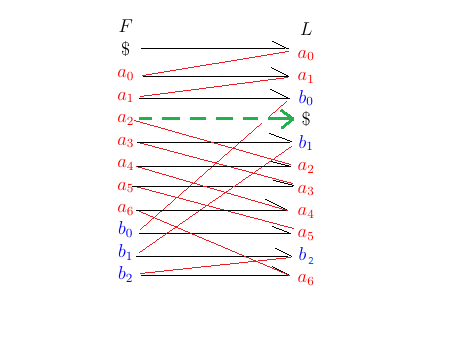
\includegraphics[width=0.5\textwidth]{bwt0}
    \captionsetup{width=0.8\textwidth}
    \caption{ From F--> L to $S$}
    \label{fig:bwt0}
\end{figure}

The FM-Index provide an opportunity for searching in compressed $bwt$ files without full decompressing, which is important for the “Big Data” era of sequencing. 
We can search in a compressed $bwt(S)$ file using FM-index. Suppose that we want to find an occurrence of pattern $P$=aab in $bwt(S)$=bc\$ababaaa, so we build a FM-index, as illustrated in Figure \?.  We search $P$ from right to left, and find all occurrences of $b$ in $F$. Luckily these are grouped together as part of the design and can be found in index 6 through 8 in $F$. Next we look at index 6 through 8 in $L$, and find any characters $c=a$, since $b$ is preceded by $a$ in $P$. Index 7 and 8 in $T$ both have $a$’s, so we look at the ranks of these, and locate the same characters in $F$ with these ranks, which is in index 3 and 4.  Then we find occurrences of $a$ at index 3 and 4 in $L$, since $a$ is preceded by $a$ in $P$. $P$ is now exhausted, and we can therefore confirm that there is an occurrence of $P$=aab in $bwt(S)$=bc\$ababaaa.  This searching approach find the number of all occurrences of $P$ in $bwt(S)$, but it does not tell us where in the text these occur. 
FM-index using bwt is a sort of a suffix array, but is easier to compress. 


\subsection{Application}

We have seen two static datastructures, here the suffix tree and the space efficient suffix array, both which can be constructed in linear time complexity and searched in $O$(n) and $O$(n log m), respectively. Now we tend to the question regarding applications and operation, here if suffix trees and suffix arrays can be used in the same applications and supports equal operations. 

The suffix tree is undouptly one of the most important datastructures in string processing and comparative genomics and once constructed, can efficiently solve a myriad of string processing problems, as demonstrated by Gusfield with almost 70 pages devoted to applications on suffix tress \cite{gusfield, enchancedsuffix}. The application demonstrated by Gusfield can be classified into three kinds of traversals \cite{enchancedsuffix}:
\begin{itemize}  
\item a buttom-up traversal of the complete suffix tree 
\item a top-down traversal of a subtree of the suffix tree 
\item a traversal of the suffix tree using suffix links 
\end{itemize}
Figure \ref{fig:traversalenchanced} shows some of the application discussed in Gusfield, with their traversal kind. Although suffix trees are asymptotically linear and plays a huge role in datstructure algorithmics, they are not as widespread in todays software application as expected. There are a few reasons for that. Space consumption of suffix tree are large and act as a bottleneck in large scale applications, since they require 20 bytes per input character. Moreover, it suffers from poor locality of memory references, which causes significant effeciency loss on cached processor architectures and makes it difficult to store in secondary memory \cite{enchancedsuffix}. In several geonem analysis and geonem comparison applications the above problems have been identified for suffix trees. But as seen, a more space effecient datastructure exist, hence the suffix array which only consumes 4$n$ bytes per input character\cite{enchancedsuffix}.   
 
Mohamed Ibrahim Abouelhoda \emph{et al.} \cite{enchancedsuffix} show that \emph{every} algorithm that uses suffix trees as data structure, can systematically be replaced with an enchanced version of a suffix array (enchanced suffix arrays) and furthermore, solve the same problems in same time complexity. Enchanced suffix array is a datastructure consisting of the suffix array, and some other information or additional tables. Futhermore, enchanced suffix arrays are fast and easy to implement \cite{enchancedsuffix}.

\begin{figure}[H]
    \centering
    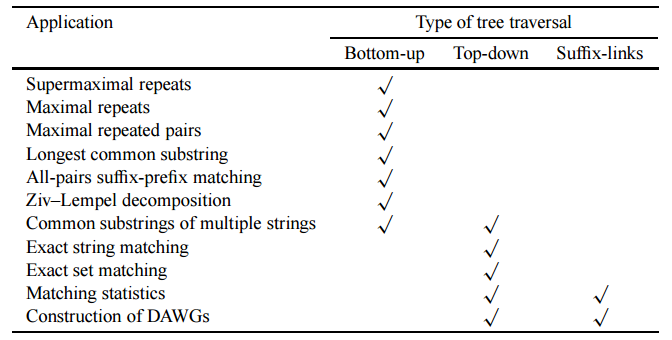
\includegraphics[width=0.5\textwidth]{traversalenchanced}
    \captionsetup{width=0.8\textwidth}
    \caption{Application on suffix trees and their traversal kind \cite{gusfield, enchancedsuffix}.}
    \label{fig:traversalenchanced}
\end{figure}

At this time it is now clear how every algorithm using a sufix tree, can be systematically replaced by an algorithm based on suffix arrays \cite{enchancedsuffix}. So we look at how enchanced suffix arrays conquer the three kinds of travesals which were classified earlier and whos applications we see in Figure \ref{fig:traversalenchanced}.
\\ \\
\textbf{Buttom-up traversal}
\\ \\
We will first look at problems that are usually solved with buttom-up traversal, and show these can be solved with enchanced suffix arrays, using maximal repeated pairs and Zip-Lempel decomposition of a string, as examples \cite{enchancedsuffix}.
\\
Maximal repeated pairs plays an important role in genome analysis, and the algorithm presented by Gusfield was implemented in the \emph{REPuter}-program \cite{gusfield, enchancedsuffix}. \emph{REPuter}-program uses maximal repeated pairs to find approximate repeats in O($\|\Sigma\| n + z$) time, where $z$ is the number of maximal repeated pairs and is based on space effecient suffix trees \cite{enchancedsuffix}. Repetitative structures are seen in the field of biology (but not limited to), where genetic mapping requires the identification of certain markers in a DNA that is variable between individuals, called tandem repeats. What varies, is the number of times a substring repeats in an array, refered to as \emph{variable number of tandem repeats} (VNTR) \cite{gusfield}. The VNTR markers are used during the genetic level to search for specific defective genes or used in forensic DNA fingerprinting, since a small set of VNTR can uniquely charactirize an individual in a population \cite{gusfield}. 

\begin{quote}
\textbf{Definition} \\
A maximal pair in a string $S$ is identical sbstring pairs $\alpha$ and $\beta$ such that the character at the immidiate left (right) of $\alpha$ is different from the character to its immidiate left (right) of $\beta$. So extending $\alpha$ or $\beta$ in any direction would destroy the equality of both strings \cite{gusfield}. 
\end{quote}

\begin{quote}
\textbf{Definition} \\
A maximal pair (or maximal repeated pairs) is given by the triple ($p_1, p_2, n'$), where $p_1$ and $p_2$ is starting positions for two substrings and $n'$ is their length. We define $R(S)$ as the set of all triples of maximal pairs in $S$ \cite{gusfield}.
\end{quote}

Given string $S$ = $xabcyiizabcqabcyrxar$, there are three occurrences of the substring $abc$. The first and third occurrences of $abc$ do not form a maximal pair, but the first and second form the pair (2, 10, 3), and the second and third forms the pair (10, 14, 3). Note that the definition allow maximal pairs to overlap each other, so to model that case we assume that $S$ has a symbol attacted to the start and end that exists nowhere else in $S$ \cite{gusfield}.


\begin{quote}
\textbf{Definition} \\
A maximal repeat $\alpha$ is defined as a substring of $S$ that occours in a maximal pair in $S$, hence $\alpha$ is a maximal repeat in $S$ is there is a triple ($p_1, p_2, |\alpha|$) $ \in R(S)$  and $\alpha$ occurs in $S$ at startposition $p_1$ and $p_2$. We define $R'(S)$ as maximal repeats in $S$ \cite{gusfield}.
\end{quote}

In the given string $S$ = $xabcyiizabcqabcyrxar$, both $abc$ and $abcy$ are maximal repeats. Gusfield presents a algorithm using suffix trees, that finds all maximal pairs in O($n$) time for a string of length $n$ and we presented the definition for such pairs \cite{gusfield}.
\\
To compute maximal pairs, the implementation presented by Mohamed Ibrahim Abouelhoda \emph{et al.} \cite{enchancedsuffix} requires three tables: \emph{suftab}, \emph{lcptab} and \emph{bwttab}. The \emph{bwttab} contains the Burrows and Wheeler transformation (Section \ref{Burrows-Wheeler Transform}),  \emph{lcptab} contains the  longest common prefix (Section \ref{LCPsection}, though here it is a tree representation), \emph{suftab} is the suffix array (Section \ref{Suffix Arrays Section} and \ref{SAIS Section})\cite{enchancedsuffix}. These tables are accessed in sequencial order, which leads to an improved cache coherence and reducing running time, such that maximal repeated pairs can be computed in O($|\Sigma|n + z$)  time \cite{enchancedsuffix}. Mohamed Ibrahim Abouelhoda \emph{et al.} \cite{enchancedsuffix} and Kasai \emph{et al.} \cite{Kasai} proved that it is posible to compute maximal repeated pairs with suffix arrays and some additional information. We will not dwell into the algorithm for computing maximal repeated pairs, we use this to emphecies that suffix arrays can be used in the same applications which usauly solve problems with buttom-up traversal on suffix trees. Although as an example, we will show how to compute the Ziv-Lempel decomposition using suffix arrays, which is a lossless compression algorithm \cite{LempelZiv}.

\begin{figure}[H]
    \centering
    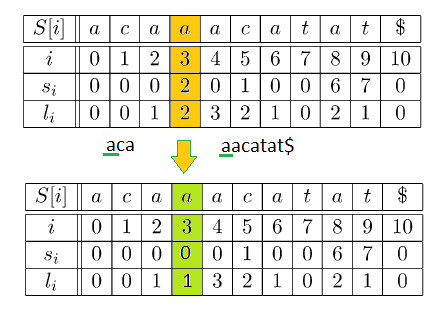
\includegraphics[width=0.4\textwidth]{LempelWrong}
    \captionsetup{width=0.8
    \textwidth}
    \caption{}
    \label{fig:LempelWrong}
\end{figure}

We follow the example conducted by Mohamed Ibrahim Abouelhoda \emph{et al.} doing a Ziv-Lempel decomposition of the string $S$=acaaacatat\$, but with a minor correction. Mohamed Ibrahim Abouelhoda \emph{et al.} claim that there exist a prefix of $i$=3 of $S$ where $l_i$=2 is the longest prefix of S[$i \ldots n$] that is also a substring of $S$ starting at some position $j < i$, hence S[$0 \ldots i-1$]. So S[$3 \ldots n$] = aacatat\$ and S[$0 \ldots$ 2]= aca, which must mean that the longest prefix of S[$3 \ldots n$] which is also a substring of [$0 \ldots$ 2] have to be $a$, with a length of 1, hence $l_i$=1 and $s_i$=0 and not $l_i$=2 and $s_i$=2 as claimed. This correction should yield the Ziv-Lempel decomposition in Figure \ref{fig:Lempeltrue} \cite{enchancedsuffix}.

\begin{figure}[H]
    \centering
    \includegraphics[width=0.4\textwidth]{Lempeltrue}
    \captionsetup{width=0.8
    \textwidth}
    \caption{Ziv–Lempel decomposition of $S$=acaaacatat \cite{enchancedsuffix}.}
    \label{fig:Lempeltrue}
\end{figure}

An interesting application of suffix trees is the $lca$ (Lowest Common Ancestor) problem, that is, finding the lowest common ancestor of node $i$ and $j$ in tree $T$. 
Lowest common ancestor was first obtained by Harel and Tarjan (1984, published online 2006 \cite{lcaWeb}) and later on simplified by Schieber and Vishkin (1988, published online in 2006 \cite{lcaWebSch})\cite{gusfield}.
\newline
Lowest common ancestor is an interesting application given that it is used in application as exact matching with wild cards and the $k$-mismatch problem, amongst others \cite{gusfield}. More interesting is the fact that $lca$ of leaves $i$ and $j$ identifies the longest common prefix of suffixes $i$ and $j$, which will be discussed later on.
\newline
By consuming linear time amount of preprocessing a suffix tree, that is a rooted tree, any two nodes can be identified and their $lca$ can be found in constant time, $O(1)$ \cite{gusfield, lca}. This paper will not dwell into the different linear time preprocessing algorithms for the $lca$ predicament, but delivers an overview and clarification of the problem by introducing a simpler but slower algorithm. (maybe linear in the appendix?).
\begin{quote}
\textbf{Definition}   In a rooted tree $T$ a node $u$ is an ancestor of node $v$, if $u$ is an unique path from the root to $v$ \cite{gusfield}.
\end{quote}
\begin{quote}
\textbf{Definition}   In a rooted tree $T$, the lowest common ancestor of two node $u$ and $v$, is the deepest node in tree $T$ that is an ancestor of both $u$ and $v$ \cite{gusfield}.
\end{quote}
Let’s suppose for simplification that an application is allowed preprocessing time of an upper bound of $\theta (n lg n)$, which is an acceptable bound for most applications \cite{gusfield}. Then, in the preprocessing state of tree $T$, perform a deept-first traversal of tree $T$ and create a list $L$ of nodes in order as they are visited. Then locating the $lca$ of node $2$ and $8$, $lca[2,8]$, in \cref{fig:travesal}, one only have to find any occurrences of $2$ and $8$ in $L$. Then take the lowest value in interval between $L[1] = 2$ and $L[12]=8$. This value is the lowest common ancestor for node $2$ and $8$ in $T$, $lca[2,8]=1$.
\begin{figure}[H]
    \centering
    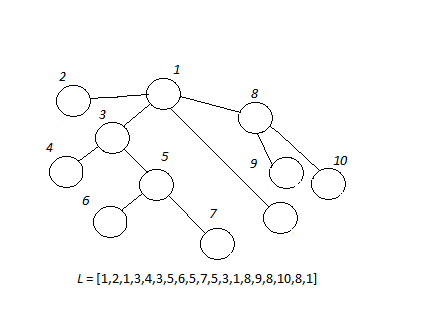
\includegraphics[width=0.5\textwidth]{travesal}
    \captionsetup{width=0.8\textwidth}
    \caption{Rooted tree - deept-first travesal with $L = [1,2,1,3,4,3,5,6,5,7,5,3,1,8,9,8,10,8,1]$}
    \label{fig:travesal}
\end{figure}

Ibrahim Abouelhoda \emph{et al.} did an experiment with two different programs computing maximal repeated pairs, using different files (listed here \ref{FILES})\cite{enchancedsuffix}. \emph{REPuter} is based on suffix tree and \emph{esarep} is based on enchanced suffix arrays \cite{enchancedsuffix}. The result is displayed in Figure \ref{fig:ButtomUp}.
The program \emph{esarep} used almost half of the space required for \emph{REPuter} and in this case 2-3 times faster and in 4-5 times faster. This comparison emphzise the advantages of enchanced suffix arrays over suffix trees \cite{enchancedsuffix}.
\begin{figure}[H]
    \centering
    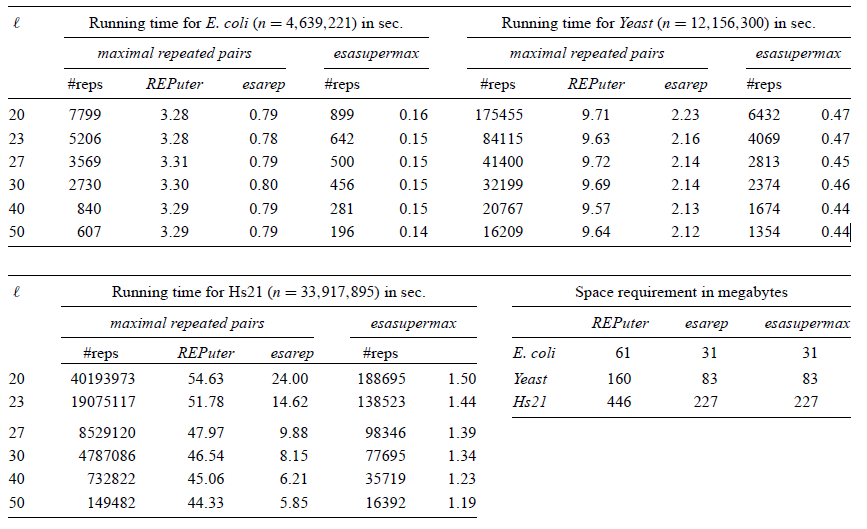
\includegraphics[width=0.7\textwidth]{ButtomUp}
    \captionsetup{width=0.8\textwidth}
    \caption{Table for computing maximal repeated pairs and supermaximal repeats. Running times are in seconds and space requirements are in megabytes. The number of repeats of length $\geq$ l is displayed in column titled \emph{\#reps}. Space requirement is independant of $l$ \cite{enchancedsuffix}.}
    \label{fig:ButtomUp}
\end{figure}
\\ \\
Top-down traversals
\\ \\
Exact string matching is usualy computed in a top-down approach when using suffix trees as datastructure as illustrated in Figure \ref{fig:traversalenchanced}.
The starting positions of $P$ in $T$ are is displayed on every leaf in the subtree below the point of the last match, demonstrated in Figure \ref{fig:ExactMatching}. We match the characters of $P$ down the unique path in $T$ until $P$ is exhausted or a character in $P$ can not be matched. So if $P$ is fully matched from the root along some path in $T$, we can find all occurrences of pattern $P$ in $T$ by buttom-up travesing the subtree below the end of the matching path and note the leaf indexs encountered. We can do this because every internal node has at least two children, so the number of leaves is proportional to the number of traversed edges \cite{gusfield}.

\begin{figure}[H]
    \centering
    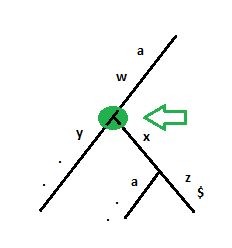
\includegraphics[width=0.2\textwidth]{ExactMatching}
    \captionsetup{width=0.8
    \textwidth}
    \caption{Suffix tree $T$ for $S$=awyawxawzz, where there are three occurrences of the pattern $P$=aw in $T$, with their positions accordingly \cite{gusfield}.}
    \label{fig:ExactMatching}
\end{figure}

Another application exploiting the top-down approach is the exact set matching, where the problem consist of locating all occurrences from a set of patterns $P_{set}$ in some string $S$, where the set is sent as an input all at once \cite{gusfield}. \\ We define a \emph{keyword tree} as:

\begin{quote}
\textbf{Definition} \\
The \emph{keyword tree} $T_{key}$ for the set of patterns $P_{set}$ is a rooted directed tree, which must satisfy three conditions:
\begin{itemize}  
\item All edges are labeled with exactly one character
\item Any two labels comming from the same node, must have distinct labels
\item Any pattern $P_i$ in $P_{set}$ maps a node $v$ of $T_{key}$ in a way that all characters from the root to node $v$ spells out pattern $P_i$ \cite{gusfield}.
\end{itemize}
\end{quote}

Suppose that we have a set of patterns $P_{set}$ = \{potato, poetry, pottery, science, school\} and its keyword tree defined as illustrated in Figure \ref{fig:KeywordTree}. Since no two labels comming from the same node have identical labels, we can use the keyword tree to search for any occurrences of $P_{set}$ in string $S$. Notice that we preprocess $P_{set}$ into a \emph{keyword tree} $P_{key}$, such that that we can find all occurrences of patterns in $P_{set}$ in $S$ by taking each position $p$ in $S$ and follow the unique path from $r$ in $T_{key}$ which matches a substring in $S$ starting at character $p$. The \empg{dictionary problem} is one of which where the set matching effeciently solves the problem. In this problem, a known set of strings, forming a dictionary is preprocessed to which a sequence of individual string is presented to the dictionary. Each of these strings is then either contained or not contained in the dictionay. The keyword tree solves ecactly that \cite{gusfield}. Mohamed Ibrahim Abouelhoda \emph{et al.} \cite{enchancedsuffix} proved that any application that uses top-down traversals on suffix trees, can be solved using suffix arrays with some extra information \cite{enchancedsuffix}. Mohamed Ibrahim Abouelhoda \emph{et al.} conducted experiments for answering enumeration queries, with three different programs: \emph{streematch} (linked list representation of suffix trees), \emph{mamy} (suffix arrays with additional buckets) and \emph{esamatch} (based on enchanced suffix arrays) \cite{enchancedsuffix}.
\begin{figure}[H]
    \centering
    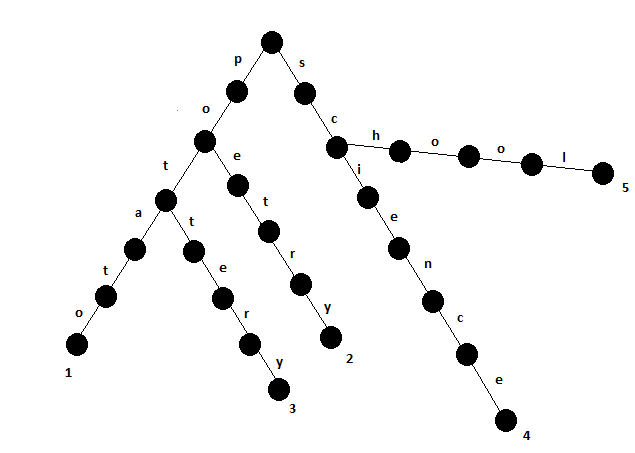
\includegraphics[width=0.5\textwidth]{KeywordTree}
    \captionsetup{width=0.8
    \textwidth}
    \caption{The \emph{keyword tree} $T_{key}$ over the set of patterns $P_{set}$=\{potato, poetry, pottery, science, school\}.}
    \label{fig:KeywordTree}
\end{figure}

The expriments were conducted on five different files listed below:
\begin{itemize} label{FILES}  
\item E. coli : The complete genome of \emph{Escherichia} bactirium (DNA) - $\Sigma$=4, length 4,639,221 
\item Yeast : The complete genome of \emph{Saccharomyces cerevisiae} (DNA) - $\Sigma$=4, length 12,156,300 
\item Hs21 : A complete collection of protein sequences - $\Sigma$=4, length 33,917,895
\item Swissprot : Complete collection of protein sequences - $\Sigma$=20, length 29,165,964
\item Shaks : A collection of the complete work of William Shakespear - $\Sigma$=92, length 5,582,655 bytes
\end{itemize}

As illustrated in Figure \ref{fig:TopDown} the program using enchanced suffix array \emph{esamatch}, outperforms all other programs in both time and space consumption, except the file \emph{Sharks}, which is explained by the large alphabet size. The program \emph{esamatch} can thereforee compete with the other programs for small alphabets \cite{enchancedsuffix}.

\begin{figure}[H]
    \centering
    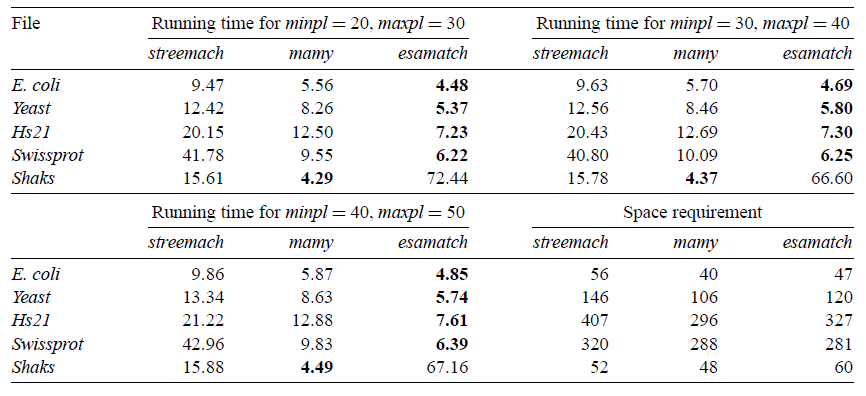
\includegraphics[width=0.8\textwidth]{TopDown}
    \captionsetup{width=0.8
    \textwidth}
    \caption{Space requirements and running times in megabytes and seconds, respectively. The programs did one million enumeration queries searching for exact patterns in the input strings. Minimal (\emph{minpl}) and maximal (\emp{maxpl}) are the minimal and maximal size of the patterns, respetively \cite{enchancedsuffix}.)}
    \label{fig:TopDown}
    
\end{figure}
\textbf{Suffix links}
\\ \\
Size of suffix trees can be reduced with the help of matching statistics, which is needed in more complex problems than exact string matching. Matching statistics are central to a fast approximate matching method designed for rapid database searching, it furthermore provide a bridge between exact matching methods and appromate string problems \cite{gusfield}.
\begin{quote}
\textbf{Notation} 
Let ms($i$) denote the matching statistics for some $i$ in string $S$
\end{quote}

Preprocess suffix tree $T$ for the fixed short string $S_p$ and keep suffix links duing the construction of the tree. We define a suffix link as:

\begin{quote}
\textbf{Definition} 
Let an arbitrary string be denoted by $x\alpha$, where $x$ is a single character and $\alpha$ a possible empty substring. For an internal node $v$ with a path label $x\alpha$, if there exists another node $s(v)$ with the path label $\alpha$, then a pointer from $v$ to $s(v)$ is a suffix link.
\end{quote}

The suffix can then be used to find sm($i$) for all $i$ in $S$. Let $S_p$ be a string of length $m$, then a matching statistics ms$i$ of $S_p$ for all $i$ in $S$, is a table of pairs ($l_p, p$), where $0 \leq j \leq m -1$ and the following holds:
\begin{itemize}  
\item $S_P[i \ldots j + t_p-1]$ is the longest prefex of $S_p[j \ldots m -1]$ that is a substring of $S$.
\item $S_p[j \ldots j + j + l_p - 1]$ = $S[p_j \ldots p_j + l_j - 1]$
\end{itemize}

Supose we have $S$= cacaccc and $S_p$=caacacacca, then we would construct the suffix tree for $S$ keeping the suffix links. Then for each position $p$ in $S_p$ we would find the length of the longest common prefix starting at some position in $S$. If $S_p[0]$=caacacacca, then the longest common prefix have length of 2 and  accour in position 0 in $S$. Next one is $S_p[1]$=aacacacca, where the length of the longest commmon prefix is 1 in $S[0]$ and $S_p[2]$=cacacca with LCP length of 4 occouring in $S[1]$. Continuing this approach we get the matching statistic table in Figure \ref{fig:matchingstatistic} \cite{enchancedsuffix}.
\begin{figure}[H]
    \centering
    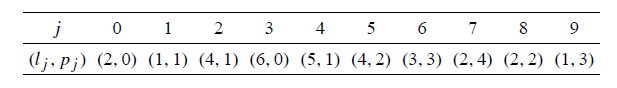
\includegraphics[width=0.6\textwidth]{matchingstatistic}
    \captionsetup{width=0.8
    \textwidth}
    \caption{Matching statistic table for $S$= cacaccc and $S_p$=caacacacca \cite{enchancedsuffix}.}
    \label{fig:matchingstatistic}
\end{figure}

The algorithm provided by Chang and Lawler \cite{enchancedsuffix} for computing matching statistic used suffix links and could solve the problem in O($n+m$) time. Later on Mohamed Ibrahim Abouelhoda \emph{et al.} \cite{enchancedsuffix} proved that any problem that used suffix links with a suffix tree datastructure, could be solved using suffix arrays with some extra information in same time complexity as the algorithm presented by Chang and Lawler\cite{enchancedsuffix}. Mohamed Ibrahim Abouelhoda \emph{et al.} performed an experiment where two programs computed the matching statistics on a pair of genomes, using a suffix tree and an enchanced suffix array as data structure, respecively \cite{enchancedsuffix}. The result displayed in Figure \ref{fig:matchingtest} revealed that \emph{esams} consumed 30-40\% less space in respect to \emph{streems}, although the latter were up to three times faster \cite{enchancedsuffix}.  

\begin{figure}[H]
    \centering
    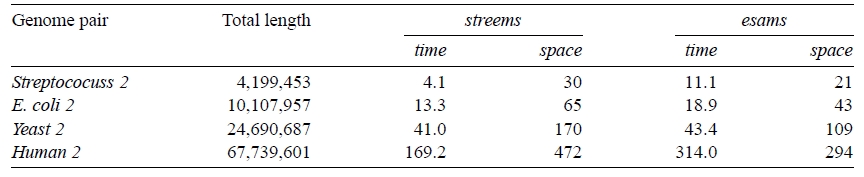
\includegraphics[width=0.8\textwidth]{matchingtest}
    \captionsetup{width=0.8
    \textwidth}
    \caption{Running time in seconds and space consumption in megabytes for matching statistics. The program \emph{streems} uses suffix tree as data structure, where the tree construction time is not included. The program \emph{esams} uses enchanced suffix array as datastructure, here a suffix array with some extra information \cite{enchancedsuffix}. }
    \label{fig:matchingtest}
\end{figure}

\subsection{SAIS-FLS - Space requirement reduction for fixed length strings}

Suppose that string $S$ consists of fixed length strings concatenated together, where each string $S_0,S_1,...,S_{n-1}$ is terminated with the sentinel $\$$ such that $S=S_0\$S_1\$...S_{n-1}\$ $.
\\ \\
Let $S=S_0\$S_1\$...S_{n-1}\$ $ consist of concatenated fixed length distinct strings, such that $|S_0|$ = $|S_1|$=…=$|S_{n-1}|$ and each string in $S$ is terminated by the sentinel.
\\ \\
Let the length of pattern $P$, $|P|$, be same length as the fixed length distinct string in $S$, such that $|P|$=$|S_0|$ = $|S_1|$=…=$|S_{n-1}|$ .
\\ \\
Suppose that the string $S=jazz\$fuzz\$quiz\$$  is given and suffix array SA for $S$ has been computed, such that $SA=[14,4,9,1,5,12,0,10,11,6,13,3,8,2,7]$ as illustrated in Figure \ref{fig:jazz}.

\begin{figure}[H]
    \centering
    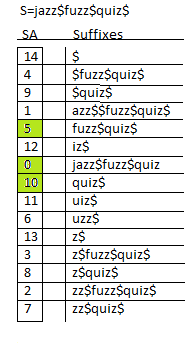
\includegraphics[width=0.2\textwidth]{jazz}
    \captionsetup{width=0.8
    \textwidth}
    \caption{Suffix array and suffixes for S=jazz$\$$fuzz$\$$quiz$\$$}
    \label{fig:jazz}
\end{figure}

By means of the Binary Search algorithm, suppose we want to find pattern $p_0=jazz\$$, $ p_1=fuzz\$$ and $p_2=quiz\$$ in the suffix array for $S$, such that $SA[i]$ pattern$ p_0=jazz\$$,$ p_1=fuzz\$$ must be a suffix of $T[SA[i]]$. Then $p_0=jazz\$$ is a suffix of $T[SA[0]]$, $p_0=fuzz\$$ is a suffix of $T[SA[5]]$ and $p_0=quiz\$$ is a suffix of $T[SA[10]]$. Now suppose, that we are only interested in exact matching, and do not care for unnecessary suffixes, then notice that we can match all fixed strings in $S$, with merely three indices in $SA$ for $S$, which leads to 12 indices in $SA$ for $S$ that are never used when exploiting exact string matching. 
\\
\begin{quote}
Let $N_DS$ denote the number of fixed length distinct strings in $S=S_0\$S_1\$...S_{n-1}\$ $, where $n$ is number of characters in $S$.
\end{quote}
\\ \\
This paper introduce an algorithm that reduce suffix array size for fixed length exact matching, from $O(n)$ to $O(N_DS)$ space complexity with linear time construction. 

\begin{quote}
\begin{lstlisting}
SAIS-FLS(string S, array SA, int len)
	let SA_FLS = new array[int]()
	for i=0 to i < length(SA) - 1 do:
		if(SA[i] NOT EQUAL TO length(S) - len
		&& S[SA[i] + len] EQUALS ''$'') 
			then PUT i in SA_FLS
	return SA_FLS
\end{lstlisting}
\end{quote}

Suppose that the length of the strings in $S$, $len$, is known, then scan $SA$ once, from left to right, and find any index where $T[SA[i] + len] = \$$ and add the elements to the new array SA-FLS in $O(m)$ time, where $m$ is the length of $SA$. Constructing the new suffix array for $S$ using SAIS-FLS, all unnecessary indices in SA are removed and the new array maintain the lexicographical order.
\\
\begin{quote}
\textbf{Lemma 6.9-1} $SAIS-FLS$ return a new array $SA-FLS$ that is sorted in lexicographical order.
\end{quote}
\\ \\
\textbf{Proof By Contradiction} 
\\ \\
Let $S$ be a string of strings, where each string is concatenated with the termination symbol $\$$. 
\\ \\
Let $SA$ be the suffix array for string $S$ and let $n$ denote the number of characters in $SA$. Suppose $SA$ is sorted lexicographical for all suffixes in $S$.
\\ \\
Suppose that S[SA-FLS[i]] to S[SA-FLS[j]], where i < j < |SA-FLS| is sorted in lexicographical order.
Suppose that $S[SA-FLS[j+1]]$ is lexicographical smaller than $S[SA-IS-FLS[j]]$, that would suggest that $SA$ for $S$ is not sorted lexicographical for all suffixes in $S$, which is a contradiction. Furthermore, since $SA$ is scanned from left to right and supposed sorted in lexicographical order, each item put in $SA-FLS$ must have been appended in lexicographical order. 
\\
\begin{quote}
\textbf{Lemma 6.9-2} $SAIS-FLS$ return a new suffix array, $SA-FLS$, containing all indices from $SA$ for $S=S_0\$S_1\$...S_{n-1}\$$ where $S[SA-FLS[i] + len] =\$$, $len = $|S_0|$ = $|S_1|$=…=$|S_{n-1}|\$$ and $0 < i < n$.
\end{quote}
\\ \\
\textbf{Proof By Contradiction} 
\\ \\
Suppose that there exist some $i$ and $j$, $i < j$, in SA, $0 < i < j < |SA|$ and $len = S_0$ in $S=S_0$$, $S_0$ =\$, where $S[SA[i] + len] = \$$ and $S[SA[j] + len] = \$$. Suppose that SA-FLS contain one item, that would suggest that $i=j$ which is a contradiction.
\\ \\
Suppose that $SA$ is sorted in lexicographically order for all suffixes in $S=S_0\$S_1\$...S_{n-1}\$$ where $S_0, S_1,…,S_{n-1}$ does not contain the termination symbol \$ and $len =|S_0|=|S_1|=…=|S_{n-1}|$.
\\ \\
Suppose that all indices from $SA$, where $S[SA[i]+ len] = \$$, $0 < i < n$, has been successfully added to the array $SA-FLS$. Suppose that there exists some $j$ in $SA-FLS$ where $S[SA-FLS[j] + len] =\$$, that would suggest that there exists an index $SA[i] = SA[j]$ where $S[SA[i] + len] =\$$, but that is a contradiction, since only indices that are bound by $S[SA-FLS[i] + len] =\$$ was added to $SA-FLS$.
\\ \\
Lemma 6.1-1 and Lemma 6.1-2 suggest that $SA-FLS$ contains indices in lexicographical sorted order and are bound by $S[SA-FLS[i] + len] =\$$. Furthermore, the length of $SA-FLS$ is proportional to the number of the fixed length distinct string in $S=S_0\$S_1\$...S_{n-1}\$$.
For large fixed length strings such as SHA1, SHA256 or MD5 hashes, $SA-FLS$ concededly reduce the number of indices stored. A string consisting of 27.000.000 MD5 hashes would produce a suffix array consisting of 27.000.000 x 33 = 891.000.000 indices, while SA-FLS contains only 27.000.000 indices, which is a reduction factor of 33. For the Sha256, the reduction factor would be 257, hence the length of the hash plus the termination symbol.

\subsection{Suffix Array Construction Algorithm (SACA) comparison}



We saw examples of preprocessing unstructured text into suffix trees and suffix arrays, examples of searching in $O(n)$ or O(n log m) time complexity and transformed strings that are easier to compress using Burrows-Wheelers Transform. We introduced an algorithm that could reduce space requirements for fixed length strings with a factor proportional to the length of the fixed length string in $S$. Space usage is a factor, since sizes of data sets in some applications, as molecular biology, data compression, data mining and text retrieval, to name a few, can be incredibly large. In many cases the alphabet size |E| is typically a fixed constant, such as ASCII E=256 or E= 4 for DNA sequences. In such cases suffix trees and suffix arrays are larger than the text by a multiplicative factor of $O=(log_{\|E\|}n)$ = $O(log n)$. To illustrate this, suppose that we have a DNA sequence of n symbols $(\|E\|=4)$ which we would store on a computer with 2n bits. A suffix array for that DNA sequence would use 4 bytes for each n words or 32 bits, which is 16 times larger than the text itself. 
The question of space usage is important in both theory and practice, since data sets can be incredibly large, especially in the “Big Data” era of next generation sequencing (SAIS-OPT). Nataliya Timoshevskaya et al. presented in 2014 a characterization and optimization of the SA-IS algorithm for suffix array construction, focusing on irregular memory access, using concepts from Burrow-Wheeler Transform, which achieves a 27\% improvement in performance on tested data on the already tuned implementation of SA-IS in the Burrow Wheeler aligner used by the bioinformatics community (SAIS-OPT). Roberto Grossi et al. presented compressed suffix arrays and suffix trees that as a concrete example could compress a typical suffix array of 100 megabytes ASCII file to 30-40 megabytes or less, while the raw suffix array would require 500 megabytes (compressed suffix trees). 

\section{Malware - Malicious Software}

The term malware spring from the two words of malicious and software, and are used to designate any unwanted software \cite{Asurveyonmalware}. Malware is also referred to as malicious software, malicious code (MC) and malcode \cite{idika2007survey}. It was defined by G. McGraw and G. Morrisett as “any code added, changed or removed from a software system in order to intentionally cause harm or subvert the intended function of the system.” and virus was defined as “ a generic term that encompasses Viruses, Trojans, Spyware and other intrusive code.” \cite{idika2007survey,Asurveyonmalware}. A more canonical example of malware include viruses, worms and Trojan Horses and are characterized by the ability of replication, propagation, self-execution and corruption of a computer system which compromise confidentiality, integrity and effect denial of service \cite{Asurveyonmalware}. The most common way of infecting a system is to transfer malware from a polluted system, using either network or local file system, to an uninfected system \cite{Asurveyonmalware}. However, the variety of known and unknown malware is key to understanding the difficult problem of detecting malware. Categorizing malware have become more complex, as new versions appear, which is a combination of those who belong to an existing category \cite{idika2007survey}. Replication and invisibility are the property and characteristic of malware, respectively. Invisibility is used to evade themselves from detection by anti-malware and replication is used to ensure existence and in some cases the replication exhaust computer recourses in the vein of RAM and hard disk \cite{Asurveyonmalware}. Malware exploit operation system vulnerabilities, software bugs and foliage itself such that it starts with the same lifecycle as the system. In other cases, malware are remotely controlled on an supplementary system, controlling the infection \cite{Asurveyonmalware}. \\
The first anti-malware program, Flushbot Plus, was invented by Ross Greenberg in 1987 and was used to prevent viruses and Trojan horses making unwanted changes to files \cite{Asurveyonmalware}. John McAfee released VirusScan(TM) program in 1989 which could detect and repair viruses simultaneously \cite{Asurveyonmalware}. Los Alamos National Laboratory developed statistic-based anomaly detector which were rule-based on statistical analysis used with anomaly detection \cite{Asurveyonmalware}. In 1990, inductive learning of sequential user patterns combined with anomaly detection was used by the Time-based Inductive Machine (TIM), masking on access matrices for anomaly detection was used by the Network Security Monitor (NSM) and the Information Security Officer’s Assistant (ISOA) deployed statistics, profile checker, and a expert system, amongst others \cite{Asurveyonmalware}. \\
Although reports claim that malware continue to grow, researchers and manufactures evolve new methods to improve techniques for building anti-malware \cite{Asurveyonmalware}, here categorizing malware into groups. Furthermore, technological solutions increase the effectiveness and performance of malware detection systems with use of cloud computing, network-based detection, web, virtual machines, agent technologies or hybrid methods and technologies \cite{Asurveyonmalware}. There are essentially two phases in the of software lifecycle in which malware is inserted, a pre-release and a post-release phase. In the pre-release phase, a internal threat or insider, usually a trusted developer within an organization, insert malicious code into software before it is released to end-users. Code inserted  after a release to its end-users, is called post-release phase. The most popular names for users or creators of malware are black-hats, hackers and crackers and could be external/internal threats, a foreign government or an industrial spy \cite{idika2007survey}. Malware creation generally employ obfuscation or behavior addition/modification, here hiding the true intention of malicious code without behavior extensions exhibited by the malware where behavior addition/modification effectively creates new malware, respectively \cite{idika2007survey}. 
Researchers suggest that reuse of code is a major component of developing malware which plays a critical role in some signature based malware detection systems, here misuse detection methods \cite{idika2007survey}. Detection systems are developed by software companies, analyze and keep track of new programs, where valid programs are put in so-called white lists and malicious programs in grey lists. The program figuring on the grey list are scanned and classified in a controlled environments. If a grey list program-analysis result in a new malware, the software company release an update for end-user product databases \cite{Asurveyonmalware}. 

\subsection{Malware naming and classes}

According to Microsoft \cite{kosmidis2017machine}, a specific malware with particular behavior can take more than one name depending on antivirus vendors naming, which depends on number of samples collected as well as the particular malware behavior \cite{kosmidis2017machine}. CARO is a common method for naming malware and is a malware naming scheme developed by antivirus companies and researchers \cite{kosmidis2017machine}. CARO does not solve the ambiguous class label problem but tries to address the incoherent labeling in general. CARO offers an universal standard for malware naming to prevent confusion between users and antivirus vendors \cite{kosmidis2017machine}. The naming scheme is as follows: \\ \\
<malware type>://<platform>/<family name>.<group name>.<infective length>.<sub variant><devolution><modifiers>
\\ \\
A structural example of using CARO is as follows (detailed illustration in Figure \ref{fig:malwarenaming}):
\\ \\
Backdoor: Win32/Caphaw.D
\\ \\
\begin{figure}[H]
    \centering
    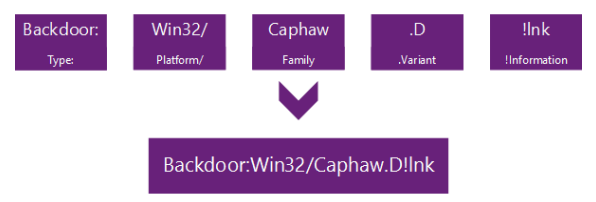
\includegraphics[width=0.6\textwidth]{malwarenaming}
    \captionsetup{width=0.8\textwidth}
    \caption{CARO naming scheme with a detailed description of a backdoor \cite{kosmidis2017machine}.}
    \label{fig:malwarenaming}
\end{figure}

Imtithal A. Saeed et al. \cite{Asurveyonmalware} divides malware into two classes: ordinary malware and network-based malware. Supplementary classifications are made depending on malware characteristics, here to facilitate authorship, correlation, information and identifying new variants. This classification is made to categorize malware into groups depending on network and web usage \cite{Asurveyonmalware}. In Figure \ref{fig:family} lists the major malware families, which is explained below.

\begin{figure}[H]
    \centering
    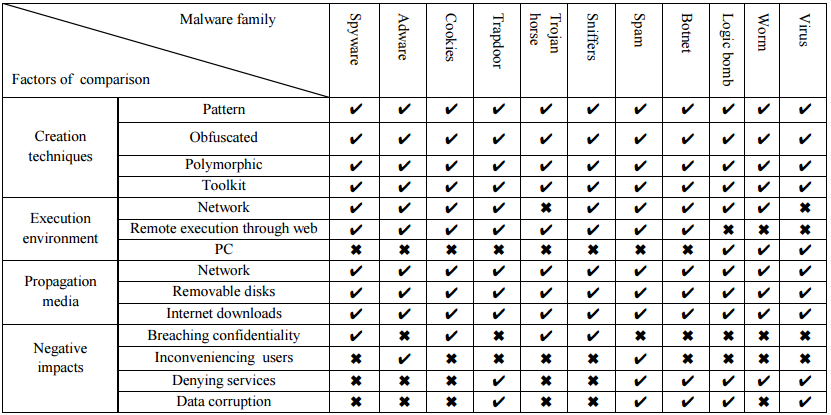
\includegraphics[width=0.8\textwidth]{family}
    \captionsetup{width=0.8\textwidth}
    \caption{A comparison scheme of major malware families \cite{Asurveyonmalware}.}
    \label{fig:family}
\end{figure}

\\ \\
\textbf{\emph{Network-based malware}}
\\ \\
\emph{Spyware:} \\
A malware installed secretly on a users computer with the purpose of gathering information without the awareness and consent of the user, is called spyware. Microsoft and Google intentionally collect information from users using their own developed spyware \cite{Asurveyonmalware}.\\ \\

\emph{Cookies:} \\
Information stored on user’s computer by their web browser with the purpose of authenticating the user depending on the information stored. Cookies stores site preferences and server-based sessions and are not executables but text formatted files. Cookies are not harmful by themselves but are in cooperation with spyware \cite{Asurveyonmalware}. \\ \\

\emph{Adware:} \\
Advertising-supported software that automatically play advertisement on user’s computer without desire. Financial profit in the main objective of adware and are not harmful, but form pop-up windows that interrupts user’s. Adware integrated with key loggers and other privacy-invasive software can though be harmful \cite{Asurveyonmalware}. \\ \\

\emph{Backdoors:} \\
Backdoors are malicious code integrated in an application or operating system with the purpose of granting programmers access to the system bypassing ordinary authentication methods. Trapdoors are a security problems because they give full access to the system without authentication and can be remotely accessed by attackers. Though backdoors are written by experts and specialized developers for friendly usage \cite{Asurveyonmalware}. \\ \\

\emph{Trojan horse:} \\
Code that appears useful but actually steals information \cite{Asurveyonmalware}. \\ \\

\emph{Sniffers:} \\
Programs that intercepts and record network traffic.  Packages are intercepted and captured, here to decode and extract raw data, to gain access to fields and their content. Information gathered this way can later be used to launch an intrusion attack \cite{Asurveyonmalware}. \\ \\

\emph{Spam:} \\
Spam is a software package that sends identical email messages to numerous email addresses. This form of spam can cripple systems, as possibly thousands emails consume bandwidth \cite{Asurveyonmalware}.  \\ \\

\emph{Botnet:} \\
A collection of infected computers which all contain embedded bot software and are controlled by a hacker. The collection of bot-infected computers are then used to execute malicious functions, bypassing any ordinary authentication that would normally be needed to acquire control of the computers. Denial-of-service (DoS) attacks uses botnet software \cite{Asurveyonmalware}.  
\\ \\
\textbf{\emph{Ordinary malware}}
\\ \\
Virus is software code that can potentially replicate itself during infection, to other applications of documents. Virus is code attached to application software using three different methods: pre-pending, embedding, and post-pending. As an example, the Autorun.inf file is target by malware developers with the purpose of replacing or adding malicious code. The Autorun.inf resign in a removable disk or storage device with the job of playing the disk or storage device automatically. Whenever a storage device or disk enters the system, the operation system searches for the Autorun.inf file and executes it. Consequently, the virus will be infecting the system as the operation system execute the Autorun.inf file \cite{Asurveyonmalware}.  Another ordinary malware, are Worms, which are self-replicating software, that does not require a host program, but work independently. Worms create copies of themselves to increase the spread rate, though this characteristic is used by antivirus scanners, to locate numerous files with identical attributes which may indicate a malware infection. Worms roaming on a server can likewise consume bandwidth, preventing normal users to access the  server \cite{Asurveyonmalware}. \\
Malicious code that remains quite until some unambiguous condition is met, typically a date and time, is called a logic bomb. Consequently, the logic bomb activates and executes when the condition is met and can have a huge impact on a systems confidentiality, or preventing online services or just sabotage files \cite{Asurveyonmalware}.  
\\
\subsection{Current threat}
\\ 
Everyday services are accessible, as web-banking, e-shopping, social media and general communication, through the internet and thus plays a vital role in our daily life. In an increasing growing and global market, the internet has become a enormous information and communication network. People do transactions and relations everyday through the internet which consequently make malware, a program that aid people achieve their malicious intentions and goals \cite{kosmidis2017machine}. \\
Developers and criminals will exploit threats and vulnerabilities as long as they exists, which seems they do not. The largest and most noteworthy  vulnerability found, was the so-called Heartbleed-bug. The bug was  discovered in the Transport Layer Security (TLS) heartbeat function and was announced in 2014 \cite{kosmidis2017machine}. TLS (SSL version 3) is an enhanced version of TCP with security services, including confidentiality, data integrity and end-point authentication \cite{kurose2010computer}. Attackers and criminals could potential exploit this vulnerability and get access to web application memory. The web application memory could potentially contain sensitive data as usernames and passwords, emails and documents \cite{kosmidis2017machine}. \\
Another recent threat for organizations and businesses is the ransomware Cryptowall which locks and encrypts all programs and files on the system and hereafter demands a pay or ransom from users or groups in order to unlock the files and programs. This payment is usually in bitcoins, which is a peer-to-peer electronic cash system that allow online payments to be sent to one party to another without going through a financial institution \cite{kosmidis2017machine} \cite{nakamoto2008bitcoin}. \\
\begin{figure}[H]
    \centering
    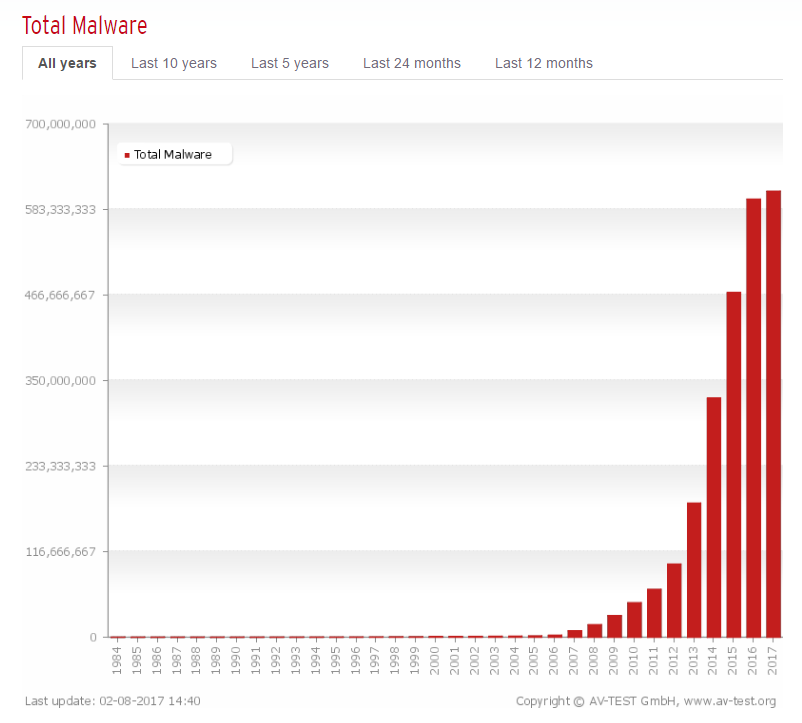
\includegraphics[width=0.8\textwidth]{totalmalware}
    \captionsetup{width=0.8\textwidth}
    \caption{}
    \label{fig:totalmalware}
\end{figure}

With the exponential growth of the internet, new malware is created every day. According to AV-TEST, an independent IT-security institute, 390.000 new malicious programs are identified each day, bringing the total malware count above 580.000.000 so far as illustrated in Figure \ref{fig:totalmalware} \cite{avtest}. It therefore imperative for security companies to detect and analyze new malware and notify users and companies about new vulnerabilities and threats \cite{kosmidis2017machine}.  
\\
\subsection{Detection techniques}
\\ 
Malware detection techniques can roughly be categorized as either anomaly-based detection or signature-based detection. Signature-based techniques scrutinize and evaluate programs against a dictionary of malware signatures in a database. The characterization of malware signatures are key to a signature-based technique and the benefit is effectiveness. The shortcoming is that signature-based techniques cannot shield against unknown malware \cite{Asurveyonmalware, idika2007survey}. Anomaly detection techniques exploit knowledge of what is constituted normal behavior to scan programs and decide the grade of maliciousness \cite{idika2007survey}. If a program violate the constituted normal behavior it is considered malicious \cite{idika2007survey}. 
The two detection techniques employ one of three different approaches: static,  dynamic, or hybrid. Each approach determine the information-gathering technique for the two categories, here the information to detect malware. The static approach uses syntax or properties of the program under inspection to determine if the program is malicious. In  a signature-based technique using static-analysis approach an attempt is done to detect if a program is malicious before it executes, while a dynamic approach would attempt to detect malicious behavior during program execution or after program execution \cite{idika2007survey}. A hybrid approach combine both static and dynamic information to detect malware \cite{idika2007survey}.
\\
\subsection{Anomaly-based detection}
\\
Two phases usually occur when exploiting anomaly-based detection, a training phase and a detection phase. In the training phase a detector attempt to learn the normal behavior and the detection phase determine if a program exhibits unwanted behavior from the normal behavior-information gathered in the training phase \cite{idika2007survey}. An ability and advantage of anomaly-based technique is to detect unknown malware, reminiscent of zero-day attacks. But this technique is not without limitations. Determining normal behavior-features during the learning phase is complex and have high false-positive rate \cite{idika2007survey}. As an example, if some exception is not seen and analyzed in the training phase, but monitored during a scanning, it could lead to a false-positive. Therefore, a system can exhibit beforehand unobserved behavior in the monitoring phase which can lead to false-positive, here categorizing a normal non-dangerous program as malicious \cite{idika2007survey}. \\
As mentioned, detection techniques can exploit three different approaches of information-gathering: static, dynamic, or hybrid. We give examples on all three information-gathering approaches for anomaly-based techniques. \\ \\
Static anomaly-based detection exploit characteristics gathered about the file structure of a program currently under examination, here to determine malicious code. This make it possible to detect malware without executing the malware program where during the training phase, derived models attempt to determine and characterize different file types on a system  based on structural composition \cite{idika2007survey}. These models are derived from learning file types generally roaming a system. Files are given predictable regular byte composition for their respective types, such that .pdf files have unique byte composition that are different from other file types, as .exe or .doc files \cite{idika2007survey}. If a file is considered to vary to much from a given model or models it is marked as suspicious and sends it to further analysis by other some other procedure where it is determined if the file is actual malicious \cite{idika2007survey}. This method is called Fileprint Analysis (n-gram) and applying 1-gram analysis to PDF files implanted with malware had a detection rates between 72.1 and 94.5 percent. Though implanted malicious code in PDF files is embedded either in the head or tail, it is still possible to embed malicious code in the middle of a PDF in such a way that it is possible to execute and open the PDF, hence deploy the malicious embedded code \cite{idika2007survey}. \\
The dynamic anomaly-based technique take advantage of information gathered during a file execution to determine malicious code. Consequently the detection phase check for inconsistencies from the information learned in the training phase. We will look at some different methods that exploit the dynamic anomaly-based technique. One approach developed by Wang and Stolfo \cite{idika2007survey} is calculation of expected payloads for each port (service) on a system. This is done by creating a byte frequency distribution which allow for a centroid model. Centroid clustering is to separate  a set of information into subsets, here to uncover the location of a centre for each subset, such that the dissimilarity distance between the information and the centre is minimized \cite{Heuristicmethods}. Each incoming payload is compared against the centroid model created during the training phase, where the Mahalanobis distance is measured between those two. A Mahalanobis distance is the distance between two distinct groups (populations). Suppose we have two groups with boys and girls, respectively. Then consider relevant characteristics between individuals of these two groups, say height or weight \cite{mclachlan1999mahalanobis}. Then we let a random vector $X$ contain the measurement made on a given individual \cite{mclachlan1999mahalanobis}. As we are interested in measuring the difference between groups the assumption is to let the random vector X have same variation about its mean, such that the difference between the groups can be considered as the mean vectors of the random vector X \cite{mclachlan1999mahalanobis}. The Mahannobis distance acquiesce a strong statistical measurement of similarities \cite{idika2007survey}. A payload under investigation is analyzed against the centroid model, measuring the Mahalanobis distance, such that a large Mahalanobis distance consider a payload malicious \cite{idika2007survey}. Wang and stolfo \cite{idika2007survey} tested their technique against three weeks of trained data. After two weeks of testing, the approach detected 57 of 97 attacks, given a success rate of approximately 60\% and a false-positive rate of under one percent \cite{idika2007survey}.
Taylor and Alves-Foss present a technique that focuses on network protocol vulnerabilities and relies on the assumption that malicious network packets tend to have large number of SYN, FIN and RST packages and low amount of ACT packages \cite{idika2007survey}. The ACT, SYN, FIN and RST bit is contained in the flag field which is in the TCP segment structure. The acknowledgment bit ACK indicate that the value carried in the acknowledgment field is valid, hence a segment contains an acknowledgment for a segment that is successfully delivered \cite{kurose2010computer}. A TCP connection is established with an end-host (server) by sending a segment with the SYN bit set to one. When the end-host receives the segment, assuming that it actually arrives, it will extract the TCP SYN segment from the datagram, allocate variables and TCP buffers to the connection and hereafter send a segment to the client which grants connection \cite{kurose2010computer}.  Within this segment the acknowledgement field of the TCP header is set to $client\_isn+1$. When the client receives the access-granted segment from the end-host, it too allocate variables and TCP buffers to the connection. The client sends yet another segment, this time setting the flag field of the TCP header to $server\_isn+1$ and the SYN bit to zero and this segment can potential carry client-to-server data in the payload \cite{kurose2010computer}. This connection procedure is often referred to as a three way handshake \cite{kurose2010computer}. The RST bit is used  to close a connection when it is not feasible to perform a three way handshake \cite{deri2000practical}. Taylor and Alves-Foss used Mahalanobis distance between known attack clusters and normal clusters on FTP, HTTP and SMTP data. Some attacks were easily found whereas others seemed to match some of the generated clustered \cite{idika2007survey}. \\
Boldt and Carlson took a different approach, here using computer forensic methods to detect privacy invasive software whereas Adware and Spyware are the primary types \cite{idika2007survey}. The approach consist of creating a clean system, hence a system that is free of privacy invasive software. Then a snapshot of the clean system is considered the baseline for the system in question. When the system baseline is recorded, the system is exposed to privacy invasive software and regular snapshot are recorded. Boldt and Carlson accessed Ad-Ware, the most popular privacy invasive software removal tool at the time and though their technique they found that Ad-Ware found false positives as well as false negatives \cite{idika2007survey}. \\

Lastly we look at hybrid anomaly-based detection method, which combine static and dynamic anomaly-based detection. A specific malware type referred to as “ghostware” endeavors to stay invisible by deleting itself from the operating system querying utilities. Whenever an user performs a command to list a directory, the malware intercept the command-list of files, and modify it in such a way that it does not figure on the list and therefore is invisible to the user and cannot be found by Windows Application Programming Interface  (API) queries \cite{idika2007survey}. The  stream of API calls are essential equivalent to a program’s execution flow, and facilitate user mode processes to services embedded in the kernel of Microsoft \cite{ahmed2009using}. API calls can be made to different functional categories, as registry, memory, sockets, ect. Each API call has an distinctive name, a set of arguments and a return value, where the number and type can vary for dissimilar API calls \cite{ahmed2009using}. Wang et al. \cite{idika2007survey} used an inside-the-box and  an outside-the-box approach. The basic idea is to compare low-level system calls with high-level system calls. A inside-the-box approach performs both a low-level and high-level scan  within the same machine. With the outside-the-box approach, a clean host performs a low-level system call without the target host knowing. Then a high-level scan is performed, if there are any differences between the low-level and high-level scan, in either the inside-the-box or the outside-the-box approach, there is a presence of ghostware \cite{idika2007survey}. The inside-the-box approach did not utilize any false positive, whereas  the outside-the-box approach produced some false-positives. Wang et al. \cite{idika2007survey} used ten ghostware in the experiment \cite{idika2007survey}.
\\
\subsection{Signature-based detection}
\\
Malware signatures are strings of bytes that are unique for that particular malware program \cite{ye2007imds}. These signatures are then used to recognize particular malicious software which resign in e.g. executable files, boot records, or memory with a diminutive amount of false positives \cite{ye2007imds}. In respect to its anomaly-based cousin, signature-based detection are easier to implement and configure \cite{kruegel2003using}. This consequently entail that most commercial systems exploit signature-based  detection as part of their implementation \cite{kruegel2003using}. As declared, anomaly-based detection methods have the advantage of being able to detect zero-day attacks, whereas signature-based detection handle these attacks inadequately. However, anomaly-based detection comes with a cost of dealing with a high number of false-positives \cite{kruegel2003using}. Signature-based detection require a repository consisting of information accumulated from known malware signatures \cite{kruegel2003using, idika2007survey}. This repository is then searched to assess if a given program have a malicious signature/signatures stored within the repository \cite{idika2007survey}. Human expertise is exploited in creating malicious signatures and once created, the information is appended to the signature repository \cite{idika2007survey}. As with anomaly-based detection, signature –based detection employ three different approaches: static, dynamic and hybrid \cite{idika2007survey}.
\\ \\
In static signature-based detection, a program is inspected for sequences of code that could reveal suspicious malicious behavior or intent \cite{idika2007survey}. Malicious signatures are in general represented by sequences of code and the signature-based detection exploit the knowledge of this, and compare the program in analysis with the information stored in the repository. A programs maliciousness can be precisely determined without execution, which is a major advantage \cite{idika2007survey}. \\
Static Analysis for Vicious Executable (SAVE) is a method proposed by Sung et al. \cite{idika2007survey}. Sequences of Windows API calls are represented as a signature for a given virus. The distance (Euclidean distance – a distance between objects in multidimensional space \cite{deza2009encyclopedia, clusteranalysis}) is calculated between known signatures and the sequence of API calls from the suspicious program \cite{idika2007survey}. The repository is then searched using three similarity functions, measuring the similarity of the grogram’s API calls against the signatures stored in the repository. A ten percent difference (or less) will result in flagging the suspicious program under inspection as malicious \cite{idika2007survey}. SAVE was compared against 8 malware detectors: Norton, McAfee Unix Scanner, McAfee, Dr. Web, Panda, Kaspersky, F-Secure, and Anti Ghostbusters. SAVE was the single detector that were able to detect all the variants of the malware used in the study \cite{idika2007survey}.\\
A diverse approach proposed by Kreibich and Crowcroft \cite{idika2007survey} is use of honeycomb. Honeycomb is a system that uses honeypots to generate signatures and detect malware from network traffic \cite{idika2007survey}. Honeypots are automated tools to collect malware and a methodology to lure attackers as automated malware with the intention of studying them \cite{baecher2006nepenthes}. Honeypots can be divided into two general types: low-interaction honeypots and high-interaction honeypots. Low-interaction honeypots offers limited service to a potential attacker and learns about the attack patterns and behavior. Whereas high-interaction honeypots offers a genuine system to interact with, but are more complex to setup and maintain \cite{baecher2006nepenthes}. Furthermore, high-interaction honeypots offers more detailed information about the attacker and an opportunity to learn about proceeding attacks \cite{baecher2006nepenthes}. Kreibich and Crowcroft \cite{idika2007survey} worked under the assumption that any connection or traffic which were directed to a honeycomb would be suspicious. Odd TCP flags generate a signature for the connection stream, such that the signature is the connection stream that entered a honeycomb modulo the honeycombs response to the incoming connection stream \cite{idika2007survey}. A horizontal and a vertical detection schemes are used, where incoming stream last n-th message are compared to the n-th message of all streams stored in the honeycomb, and newly arrived streams are aggregated and run though the Longest Common Subsequence algorithm as well with the aggregated form for streams stored in the honeycomb, respectively \cite{idika2007survey}. \\ \\
Dynamic signature-based detection is characterized by using information gathered during program execution to determine maliciousness. Here behavior patterns reveal maliciousness of the program under investigation \cite{idika2007survey}. \\
An example of dynamic signature –based detection proposed by Ellis et al. \cite{idika2007survey}, is worm detection using identified malevolent behavior. Four behavioral signatures are identified by means of dataflow monitoring, coming in and out from a solitary node. A signature could be when a server changes into a client, here whenever a worm propagate itself. This occur when a worm compromise a server and acts as an client to infect and spread to other systems (hosts) \cite{idika2007survey}. Alpha-in and alpha-out is other base signature, which map how worms typically sends similar information across nodes and consequently have same data flow links. Though for some servers, it is not unusually to transmit similar information, here file servers as an example \cite{idika2007survey}. Ellis et al. \cite{idika2007survey} analyzed the server-client signature and the alpha-in/alpha-out signature, and found that the server-client signature perfectly detected the worm changes, whereas the alpha-in/alpha-out would be unsupportive with an alpha value of one, with a high false-positive rate \cite{idika2007survey}. \\ \\
Last but not least, hybrid signature-based detection use both static and dynamic properties to determine maliciousness of a program \cite{idika2007survey}. Polymorph and self-encrypting viruses are designed to obscure themselves and thus prevaricate pattern patching techniques. A self-encrypting virus encrypt itself, consequently obscuring malicious patterns which would normally be detected by pattern matching detection techniques. Mori et al. \cite{idika2007survey} propose a method that decrypts a mobile polymorph and self-encrypting virus in an emulator and performs a static analysis of the system calls made by the virus payload \cite{idika2007survey}. Malicious behaviors are represented by state machines and detection policies are modeled by state machines, which is user-specified. A mobile application is considered malicious whenever a match occur. This technique effectively detected 600 virus/worm samples \cite{idika2007survey}.
\section{Implementation - Intrusion Detection}
The initial step in the process of implementing our intrusion detection system was to conduct a requirement analysis, to establish key attributes and limitations to our malware intrusion detection system (MIDS):

\subsection{Datastructure - Fixed Length Distinct Strings}

Given that most commercial antimalware systems exploit the signature-based techniques as part of their implementation \cite{kruegel2003using}, we adopt the same approach in the implementation of our MIDS. We primarily focus our attention to the static signature-based technique, hence a static data structure of unique malware signatures. First and foremost as it is easier to implement and configure \cite{kruegel2003using}.  
We were given access to VirusShare.com  [virusshare] which is a repository of malware samples.  VirusShare.com contains live malware for security researchers, incident responders and forensic analysts, but auxiliary interesting for us, VirusShare.com contains a database of over 27.000.000 MD5 hashes of feasible (not confirmed) malware. MD5 is a message digit algorithm, that takes an input and produce a “fingerprint” of that input \cite{turner2011updated}. MD5 hashes are weak in the sense of computer security, as its not recommended for digital signatures \cite{turner2011updated } and are breakable  \cite{turner2011updated, wang2005break}. Nevertheless, we can undamaged use it as unique fingerprints of malicious software, given that the chance of randomly finding two different files that produces the same MD5 hash value should be infeasible \cite{thompson2005md5}. Equipped with this knowledge, we are save in assuming that we should be able calculate the MD5 value for any file in a system,  and if the calculated MD5 hash value for the given file is represented in the signature repository, we can with (almost) certainty conclude it is malicious. But we cannot guarantee that a given signature roaming the signature repository represents a malicious software, given that we do not know how, or by whom, the malware was acquired. One way of solving this ambiguity, would be to authenticate every MD5 hash from our repository against a commercial repository, say Symantec. Nevertheless, we gave the accumulated repository from VirusShare.com  the benefit of the doubt and only checked a handful of random MD5 hashes against the Symantec repository at \href{https://www.symantec.com/security_response/glossary/define.jsp?letter=m&word=md5-hash}{https://www.symantec.com/security_response/glossary/define.jsp?letter=m&word=md5-hash}, which all checked out.
We decided to build three different data structures for our MIDS: a suffix tree, suffix array and a SQL database structure. The main goal with this approach is to compare construction time, space requirement and maintainability. The suffix tree implementation employed was found at \href{https://github.com/atillabyte/SuffixTree/tree/master/src/SuffixTree}\\
{https://github.com/atillabyte/SuffixTree/tree/master/src/SuffixTree}. For the suffix array we used an implementation of the SAIS algorithm based in Ge Nong et al \cite{twoeffecient} from \href{https://github.com/JoshKeegan/SAIS-CSharp}{https://github.com/JoshKeegan/SAIS-CSharp}. For our SQL database structure, we used Microsoft SQL Server Database File.


\subsection{Malware Detecting Scanner}


\subsection{Malware Detection Service}
Access to startup items when windows boots up - .exe is executed with the startup, and hnce it too late to detect malware

\subsection{Platform and implementation language}
According to a security report from 2015-2016 by AV-TEST, 85.39\% of all identified malware in 2015, was detected in Windows\® \cite{avtestreport }, of such we have chosen to implement our MIDS on Microsoft’s newest Windows \® operating system, hence Windows\® 10.  

\section{Experimental Results}

\section{Discussion}

\section{Future work}

\section{Conclussion}
\section{Literature list and references}
\section{Appendix}



%-----------------------------------------------------------------------------

%-----------------------------------------------------------------------------
\newpage
\appendix
\label{appendix}
\section{SAIS Algorithm run}\label{SAIS Algorithm run}
\begin{figure}[H]
    \centering
    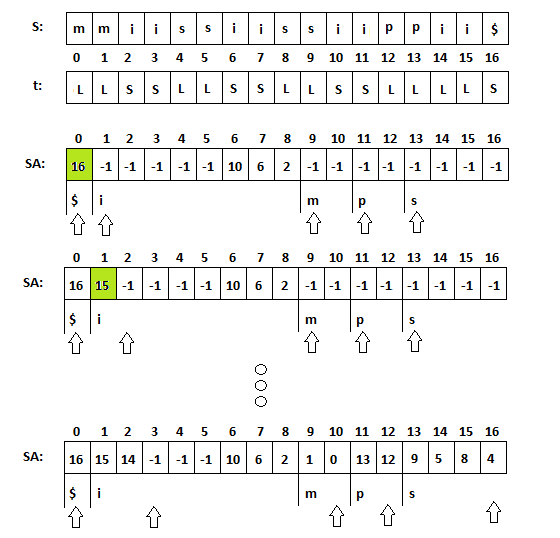
\includegraphics[width=0.5\textwidth]{SAIS_LMS2}
    \captionsetup{width=0.8\textwidth}
    \caption{$S$ is scanned from left to right, and indices for each LMS substring is appended to the end of its corresponding bucket in $SA$. The first LMS substring index is placed at the end of bucket for $i$, here at position 8 in $SA$ and forwards the bucket end one to the left, hence the bucket end for $i$ now rest at position 7 in $SA$. This process is repeated until all LMS substring indicies are placed in their buckets.}
    \label{fig:SAIS_LMS2}
\end{figure}
\begin{figure}[H]
    \centering
    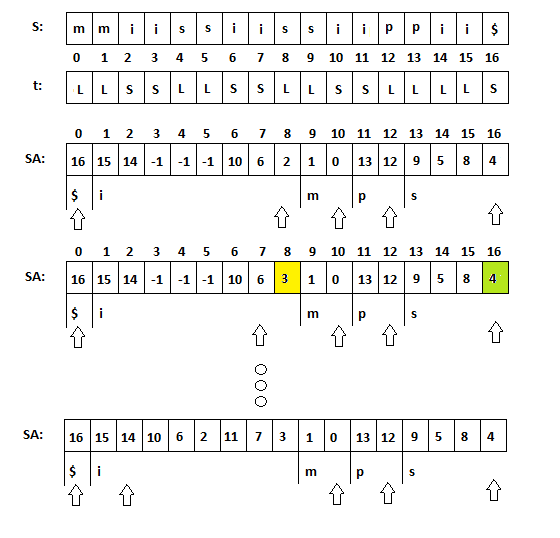
\includegraphics[width=0.5\textwidth]{SAIS_LMS3}
    \captionsetup{width=0.8\textwidth}
    \caption{$S$ is scanned from left to right, and indices for each LMS substring is appended to the end of its corresponding bucket in $SA$. The first LMS substring index is placed at the end of bucket for $i$, here at position 8 in $SA$ and forwards the bucket end one to the left, hence the bucket end for $i$ now rest at position 7 in $SA$. This process is repeated until all LMS substring indicies are placed in their buckets.}
    \label{fig:SAIS_LMS3}
\end{figure}

\newpage
\section{SAIS Recurssive step}\label{SAIS Algorithm run}
\begin{figure}[H]
    \centering
    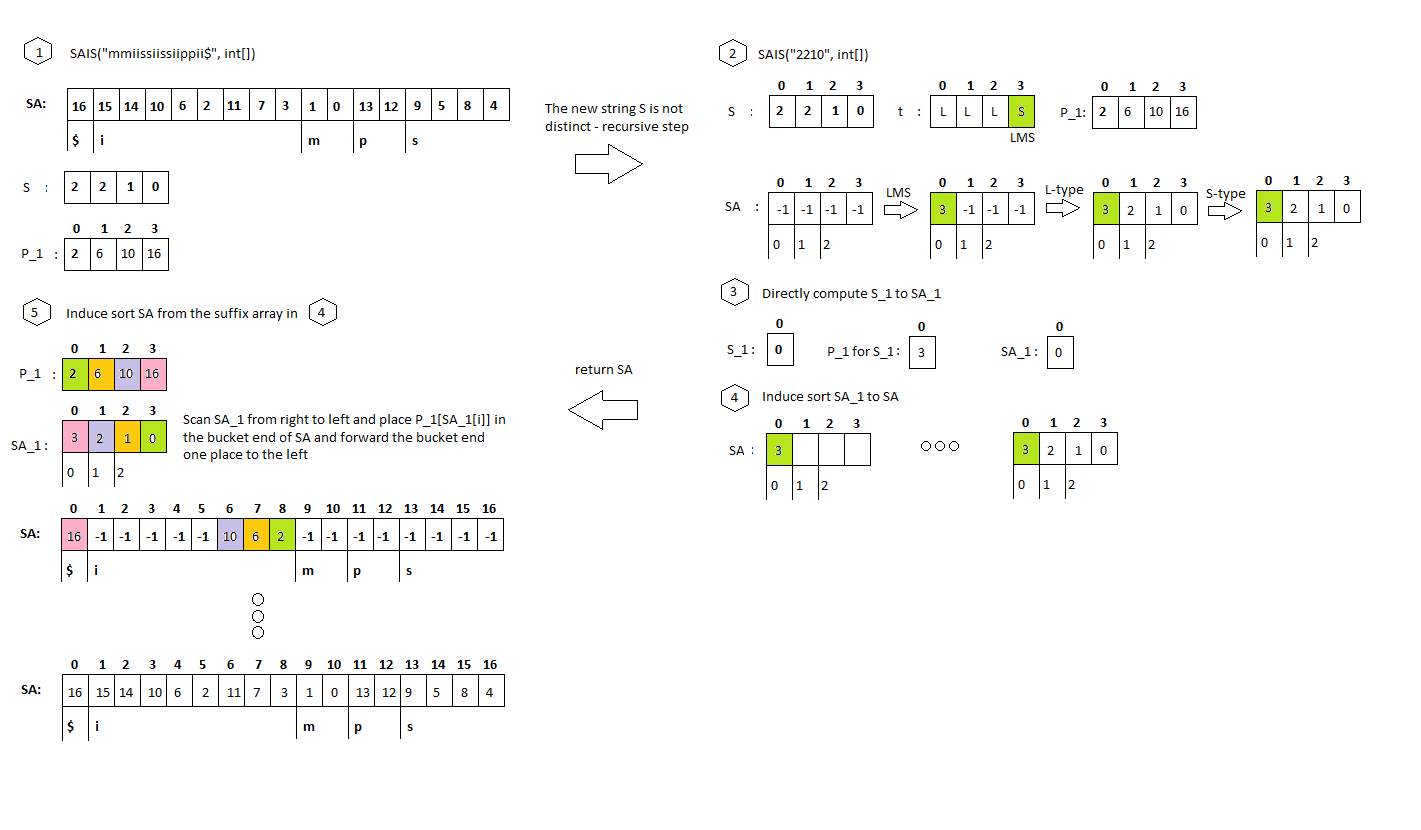
\includegraphics[width=1.1\textwidth]{SAIS_RECURSIVEDESCRIPTION}
    \captionsetup{width=0.8\textwidth}
    \caption{Some description here}
    \label{fig:SAIS_RECURSIVEDESCRIPTION}
\end{figure}
\newpage
\section{Reversing a compressed string using bwt($S$)}\label{BWT}
% THIS I WILL NOT EXPLAIN RIGHT NOW - WE CAN TAKE IT WHEN IT IS MORE RELEVANT!
\newpage
\nocite{*}
\bibliographystyle{ieeetr}
\bibliographystyle{unsrt}
\bibliography{bibliography}
%-----------------------------------------------------------------------------
\end{document}